\documentclass[11pt]{article}
\usepackage{graphicx}
\usepackage {color}
\usepackage{pdfpages}
\usepackage{float}
\usepackage{changebar}
\usepackage{enumitem,amssymb}
\renewcommand{\familydefault}{\sfdefault}
\usepackage[margin=1.2in]{geometry}
\usepackage{graphicx}
\usepackage{wrapfig}
\usepackage[super]{cite}
\usepackage{subcaption}
\usepackage[table]{xcolor}
\usepackage{amsmath}
\usepackage[sort, numbers]{natbib}

%%%%%%%%%%%%Defining the margins %%%%%%%%%%%%%%%%%%%%%
\textheight 9.in
\textwidth 6.5in
\topmargin -.5in
\oddsidemargin 0in
\setlength{\parskip}{\smallskipamount}

%%%%%%%%%%%%%%Specific Commands %%%%%%%%%%%%%%%%%%
\newcommand{\eg}{{\em e.g.,}}
\newcommand{\ie}{{\em i.e.,}}
\newcommand{\etc}{{\em etc.,}}
\newcommand{\etal}{{\em et al.}}
\newcommand{\degrees}{{$^{\circ}$}}
\newcommand{\fig}[1]{\textbf{Figure #1}}

%%%%%%%%%%%%%%%%%%%%%%%%%%%% Setting to control figure placement
% These determine the rules used to place floating objects like figures 
% They are only guides, but read the manual to see the effect of each.
\renewcommand{\topfraction}{.9}
\renewcommand{\bottomfraction}{.9}
\renewcommand{\textfraction}{.1}
\renewcommand{\familydefault}{\sfdefault} %setting the san serif font

%%%%%%%%%%%%%%%%%%%%%%%% Line spacing
% Use the following command for ``double'' spacing
%\setlength{\baselineskip}{1.2\baselineskip}
% and this one for an acceptable NIH spacing of 6lpi based on 11pt
%\setlength{\baselineskip}{.9\baselineskip}
% The baselineskip does not appear to work when we include a maketitle
% command in the main file.  Something there must set the line spacing
% If we use this next command, then things seem to work.
\renewcommand{\baselinestretch}{.9}

\setcounter{secnumdepth}{0} %make no numbers but have a table of contents


\begin{document}

\title{Lab 3, Cardiac Myocyte Simulations}
\author{Jake Bergquist, u6010393}
\maketitle
\tableofcontents
\newpage

\section{Introduction}
\par{}
Computational models of cardiac cells have been in the making for many years now, and with each development the models grow more precise, accurate, and useful.\cite{Fink2011} Mathematical and computational models of cardiac cells provide a framework for highly controlled investigation of the properties of these cells on both a single cell level and an entire organ level, comprised of a culmination of many individual cell models.  The electropysiological modeling of cardiac cells contributes greatly to an effort to integrate and interpret experimental data as well as provide a highly detailed way to perform precise and otherwise technically impractical hypothesis testing on such a fine scale.
\par{}
While there are many basic science questions and merit in the fields of computational modeling alone driving the development of more and more sophisticated and accurate cardiac cell models, one of the more practical drivers is the use of such models in exploring the effects of different diseases states and pharmacological interventions on the cardiac electro physiology. By model each cell based on the conductances of the varios ions and even at some levels the electro mechanical coupling that occurs in cardiomyocytes, investigators can assess the effects of modulating these different parameters on the function of the cell. This can guide our investigation and understanding of different disease states as well as drug development. By modeling these small scale changes such as ion conductances we can see the effects on the entire cell, and thereby the entire heart.\cite{Fink2011}
\par{}
A critical feature of such models is the ability to access and modify the various parameters that define the model on the finest scale. For this lab we are using a cardiac myocyte described by \cite{TenTusscher2003}. This mode, written in CellML and run in the JSim modeling environment, allows for the access to various parameters such as the conductances for calcium, potassium, and sodium, as well as the membrane conductance, resting membrane voltage and many other parameters. By exposing these variables the model allows us to finly investigate their interactions and the effects they have on the simulated cell. We can test various situations, such as a drug that increases the calcium conductance to 150\% of its natural value, or a disease that reduces potassium conductance to 50\% of its natural value.
\par{}
Models such as this are important for the development of our understanding not only of the field of cardiac electro physiology but also of cardiac modeling itself. By continuing to work with and develop these models, each iteration brings new precision and insight. Eventually these models all culminate in a virtual heart and eventually an entire virtual human, as is the goal of the vitrual human project.\cite{Fink2011} With these things in mind we must constantly seek to use and improve models such as this in order to lead to better tools for research and for medical treatment.

\section{Methods}
\par{}
All simulations during this lab were run using the JSim software and the Ten Tusscher Cell ML model described in \cite{TenTusscher2003}. Parameters were left at default unless otherwise stated, and figures were generated from screen capture from the JSim output. Any mathematical processing down outside of the JSim software was done using MATLAB, and the code used is appended at the end of this report in the appendix.

\subsection{1:Modeling of Repolarization}
The purpose of this section was to assess the effects of changes to the hERG potassium channel, particularly relating to the repolarization of the cell model. The simulation was run at default paprameters, then the again with the hERG conductances set to 200 \%, 50 \%, and 0 \% of the default conductance (0.0192, 0.048, 0 nanoseimens/picosecond
respectively). For each simulation the generated action potential was plotted  and captured using JSim, and the APD90 was calculated for each. The APD90 was defined as the point at which the model had repolarized 90\% to the resting value, thus it was calculated according to Equation \ref{eq:ap90} where Vb is baseline voltage, Vp is peak voltage of the action potential. The action potential duration was then calculated as the time it took from the onset of the action potential (time of maximum upstroke) till the time that the model repolarized back to the calculated AP90 voltage (time of APD90 repolarization - time of maximal upstroke). These APD90 times as well as the general action potential morphologies were compared for each of the hERG conductances.

\begin{equation} 
V(AP90) = Vb + 0.1*(Vp-Vb)
\label{eq:ap90}
\end{equation}


\subsection{2: Modeling of Calcium Transients}
\par{}
The purpose of this section was to investigate changes in calcium conductance and their effects on time to peak and calcium recovery. Fist the model was run at baseline with default parameters. Next the calcium conductance (gCal) was adjusted to 200\%, 50\%, and 0\% of the default value (0.35, 0.0875, 0
L/(faradsSeconds) respectively). The simulation was run again for each of these conductances and the membrane voltage and intracellular calcium concentrations were plotted. The time to peak was calculated in matlab by subtracting the time of the onset of the action potential (the first time point where the potential deviated from the rest value) from the time at which the action potential reached its peak. A time constant was found for the intracellular calcium recovery by curing curve fitting. Only the section of the curve after the peak was considered for exponential decay model. The time constant was calculated by importing the intracellular calcium concentration into excel and using the exponential curve fitting to fit a time constant to the data post peak.

\section{Results and Discussion}
\subsection{Potassium Conductance}
\par{}
In \ref{fig:original} we see the the JSim input and output for the default model. This model was used as a basis for all of the other work in this report. The values manipulated in this model were the the g\_Kr and g\_Cal values. All other values were left constant.

\begin{figure}[H]
	\centering
	\centering
	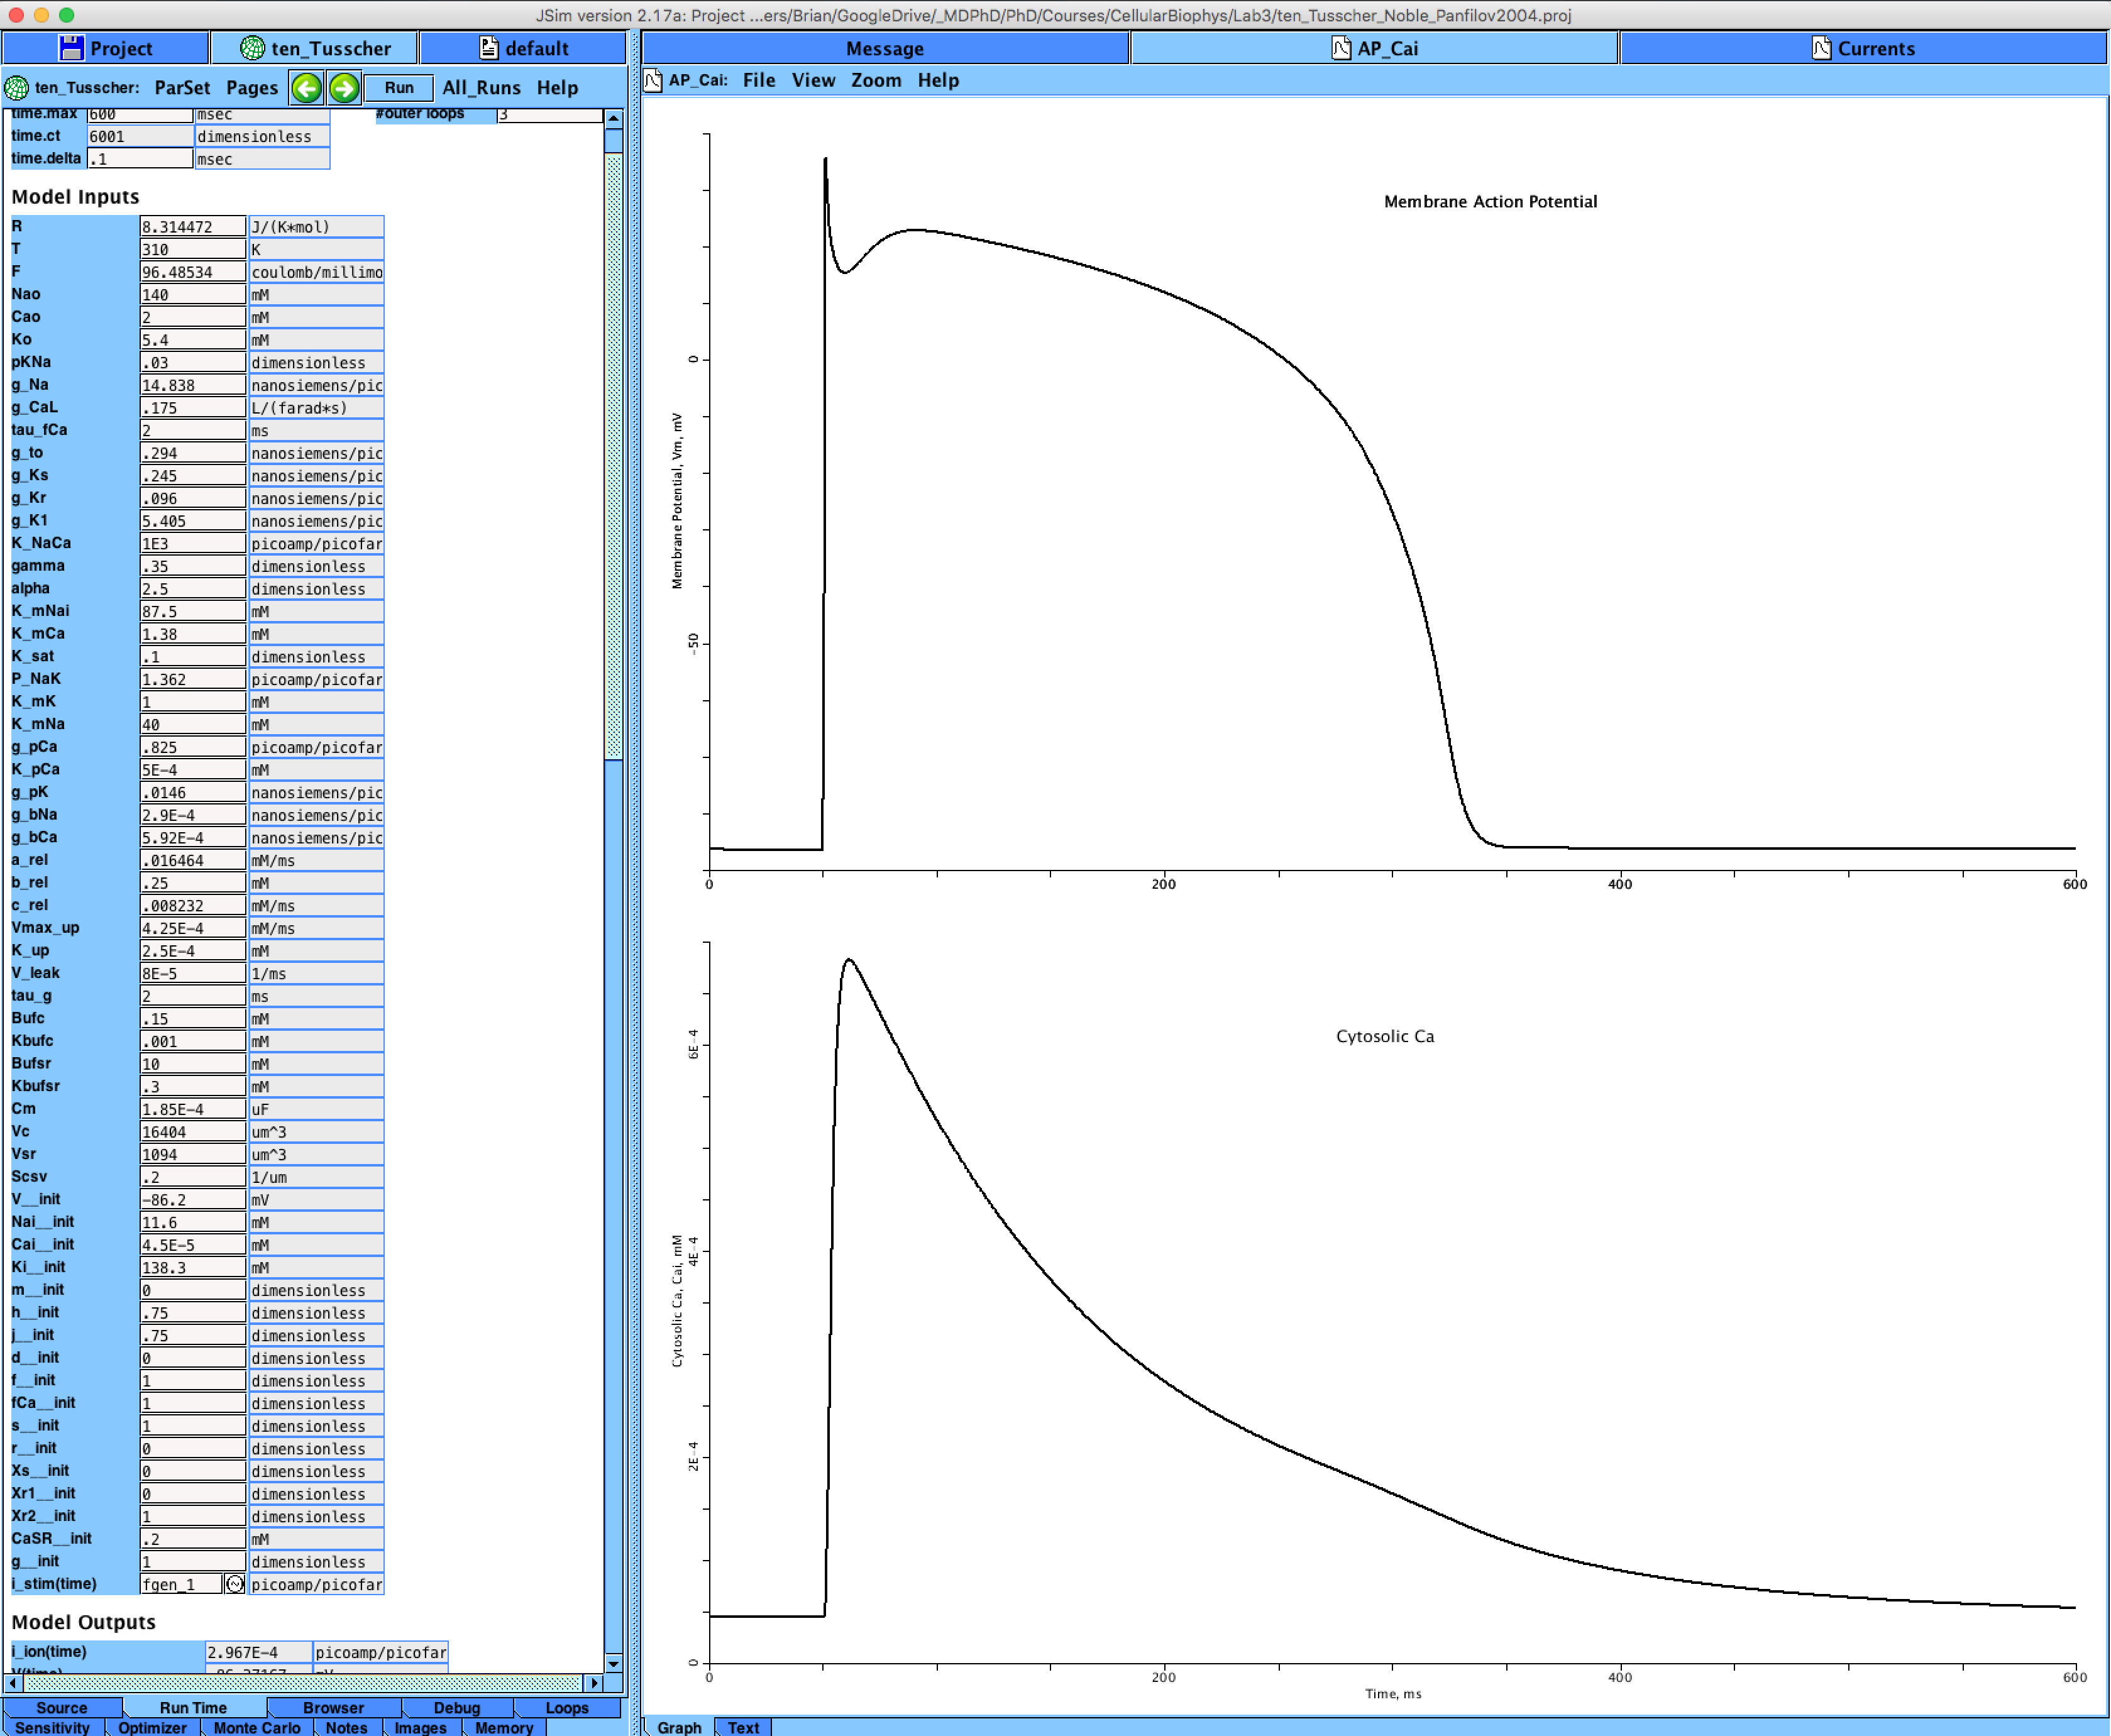
\includegraphics[width = .95\textwidth]{figs/original.png}
	
	\caption{Screen shot of JSim simulation inputs and outputs. The graphs show the simulated membrane potentials and intracellular Calcium transient. All parameters were left default for this run. }
	\label{fig:original}
\end{figure}
\par{}

In Figure \ref{fig:exp1} we see the result of altering the hERG potassium conductance (g\_Kr) on the membrane voltage. In particular we notice the change in the plateau and downslope of the action potential. Given the model, this makes sense. As hERG potassium conductance increases, the length of the action potential decreases. This is because hERG potassium is one of the main components driving repolarization of the membrane during an action potential. At lower hERG conductances, potassium cannot readily flow through the membrane and thus it cannot repolarize as quickly. At much higher hERG conductances potassium can easily flow out of the cell to cause rapid repolarization. This is seen in Figure \ref{fig:exp1} as each increase in the hERG conductance results in a decreased time to the initiation of repolarization.

\begin{figure}[H]
	\centering
	\begin{subfigure}{0.45\textwidth}
		\centering
		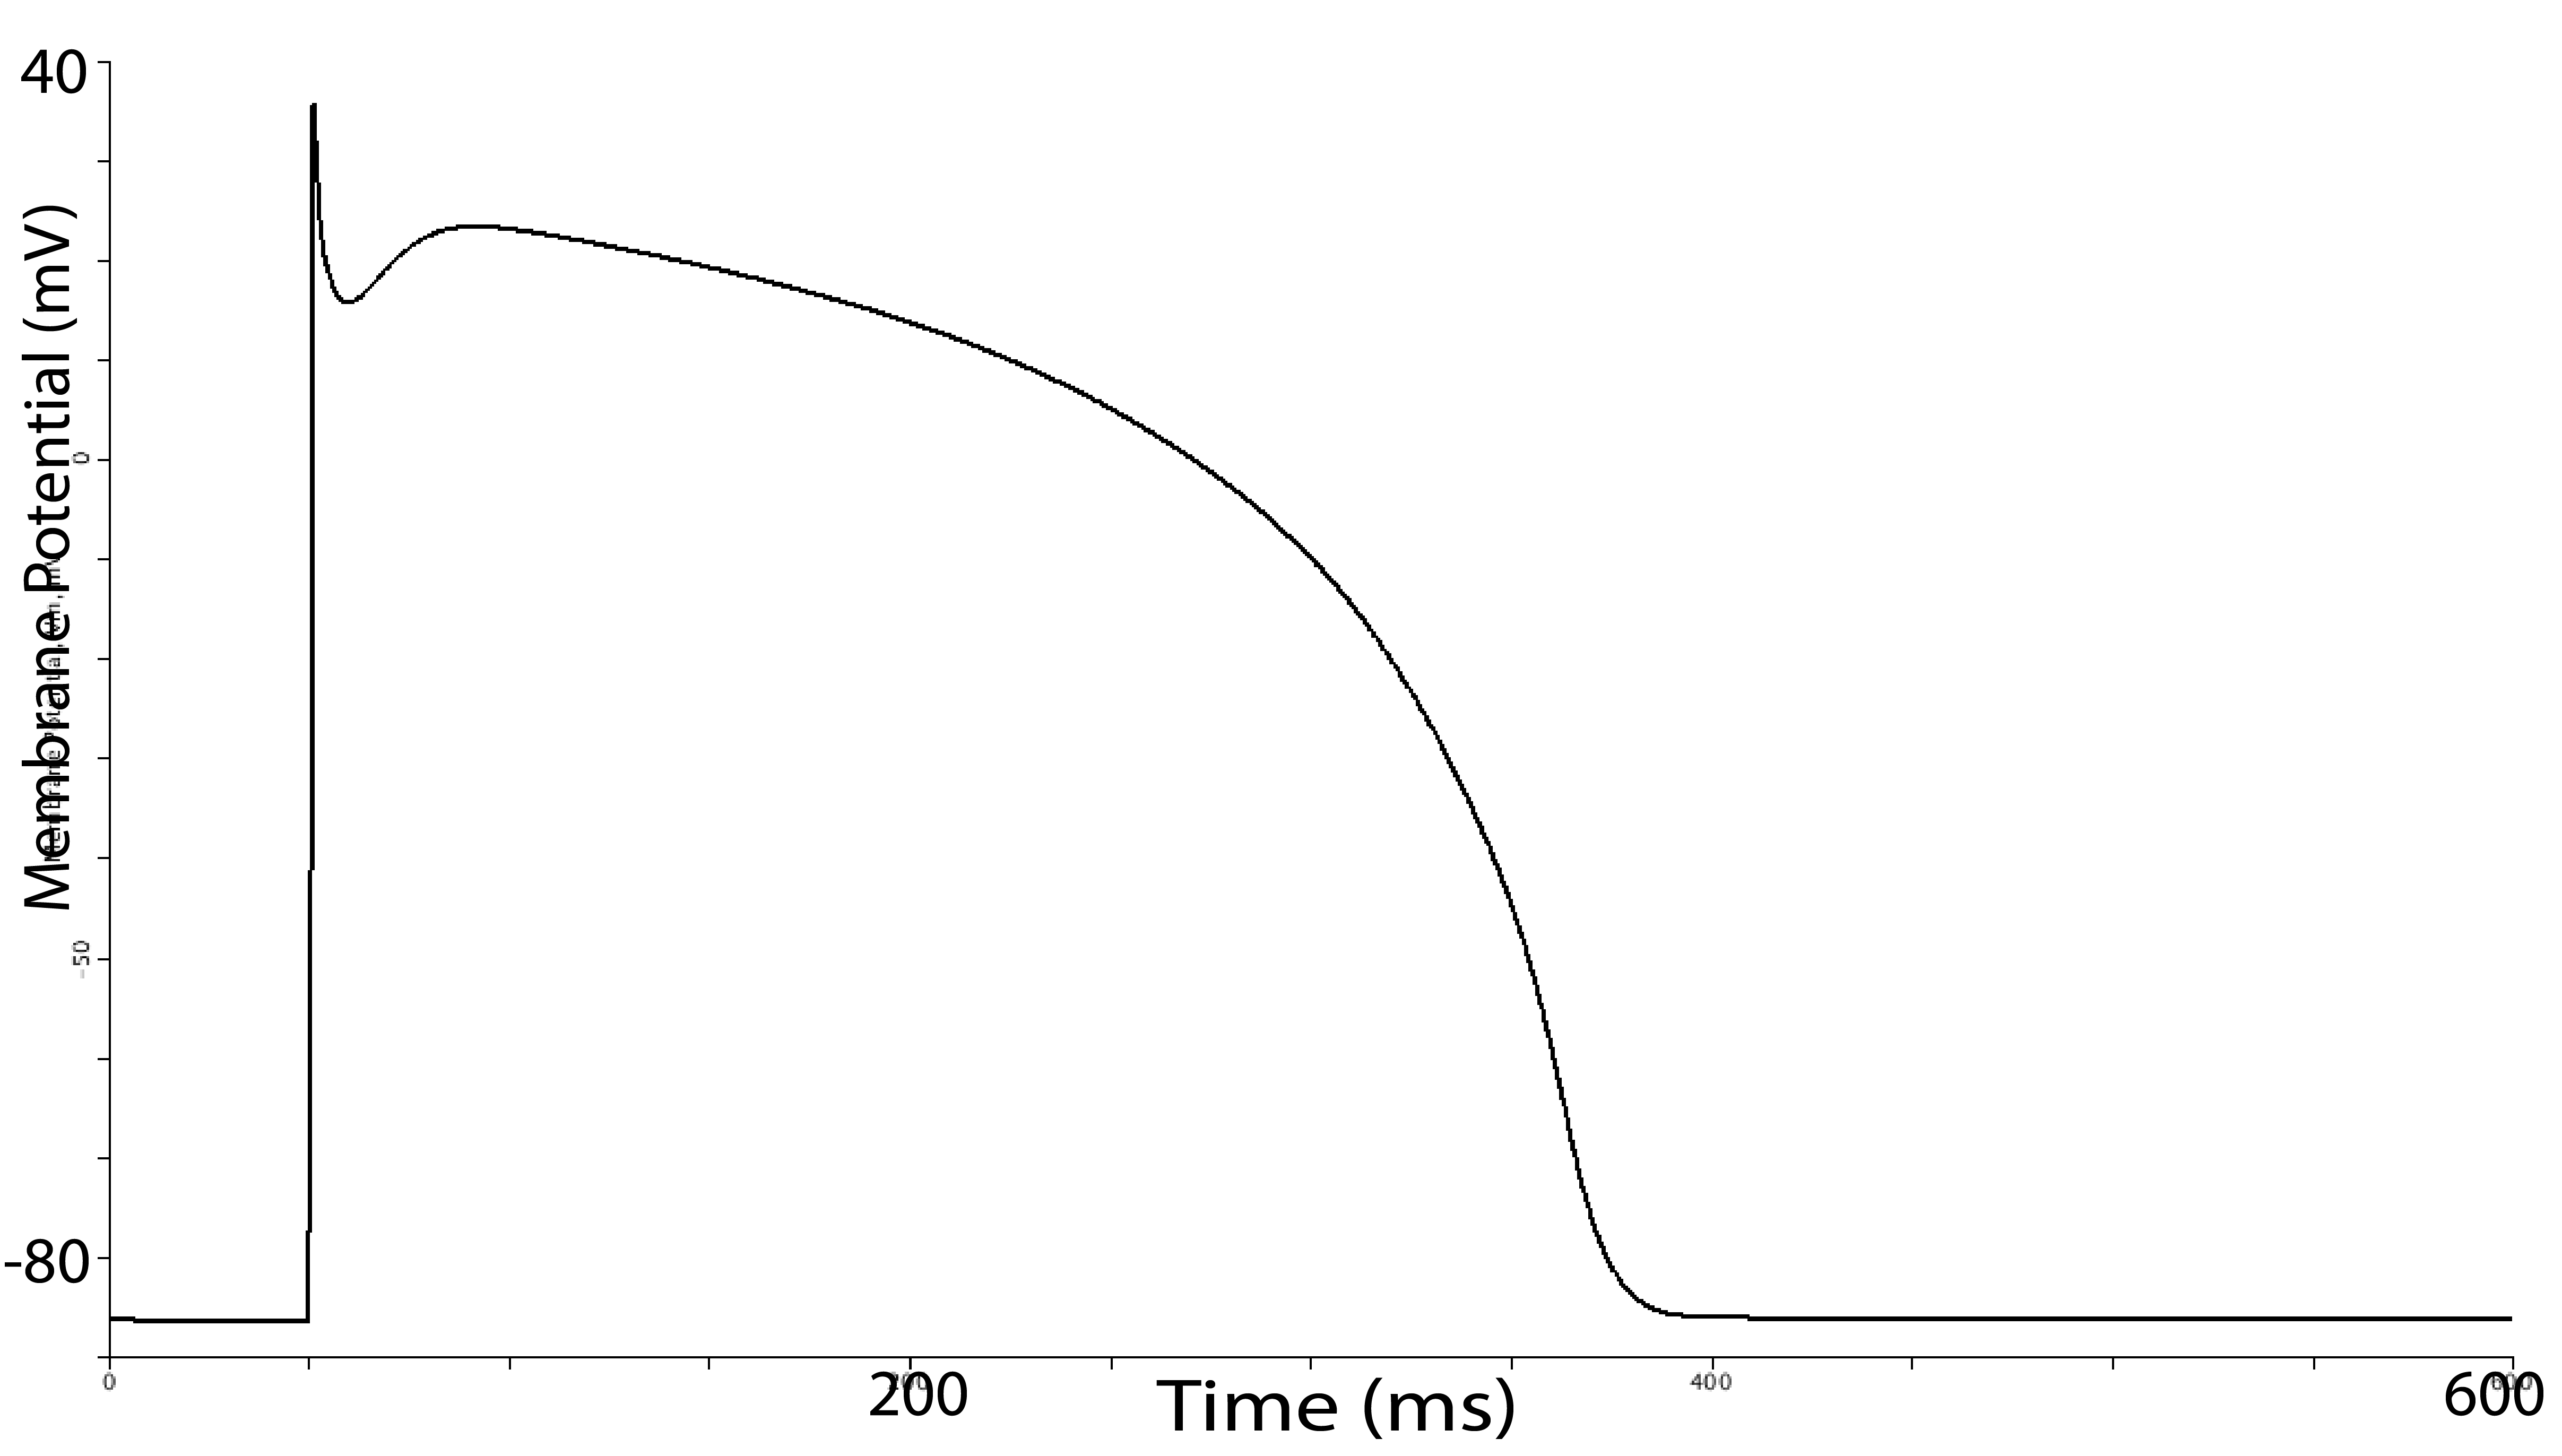
\includegraphics[width = \textwidth]{figs/0gkredit.png}
		\caption{}
		\label{exp1:a}
	\end{subfigure}
	\begin{subfigure}{0.45\textwidth}
		\centering
		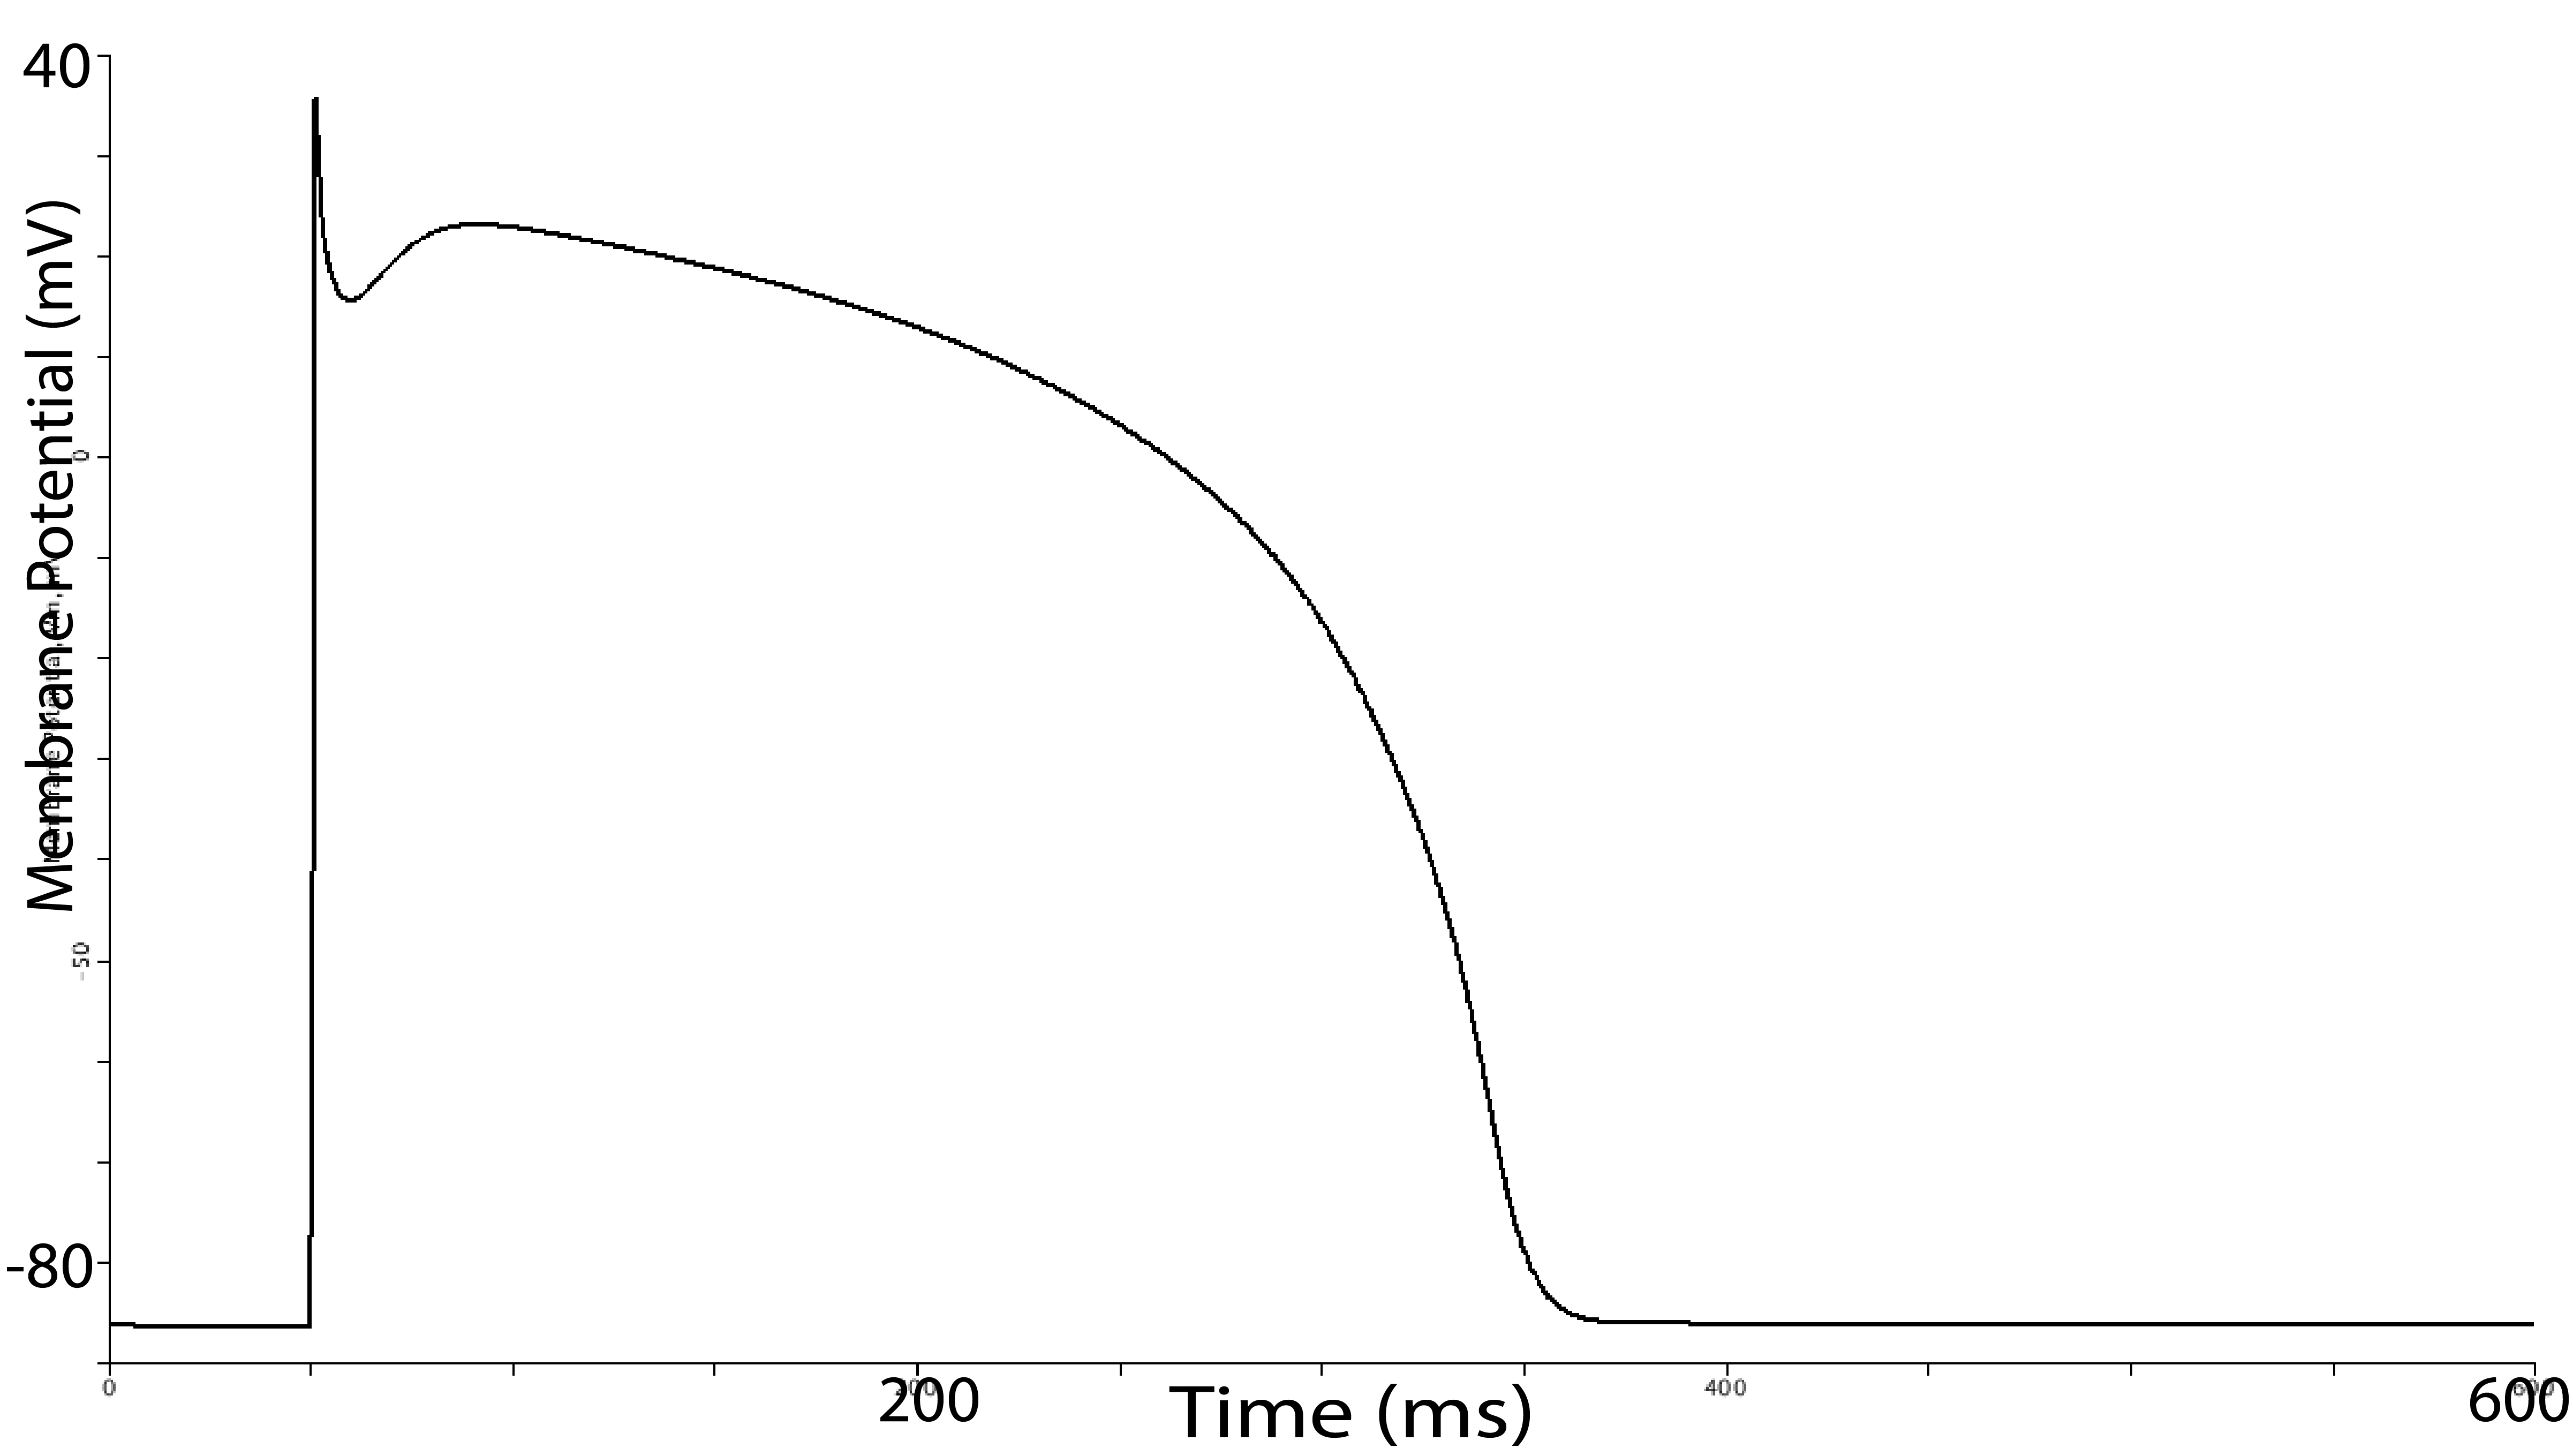
\includegraphics[width = \textwidth]{figs/50gkredit.png}
		\caption{}
		\label{exp1:b}
	\end{subfigure}
	\vskip\baselineskip
	\begin{subfigure}{0.45\textwidth}
		\centering
		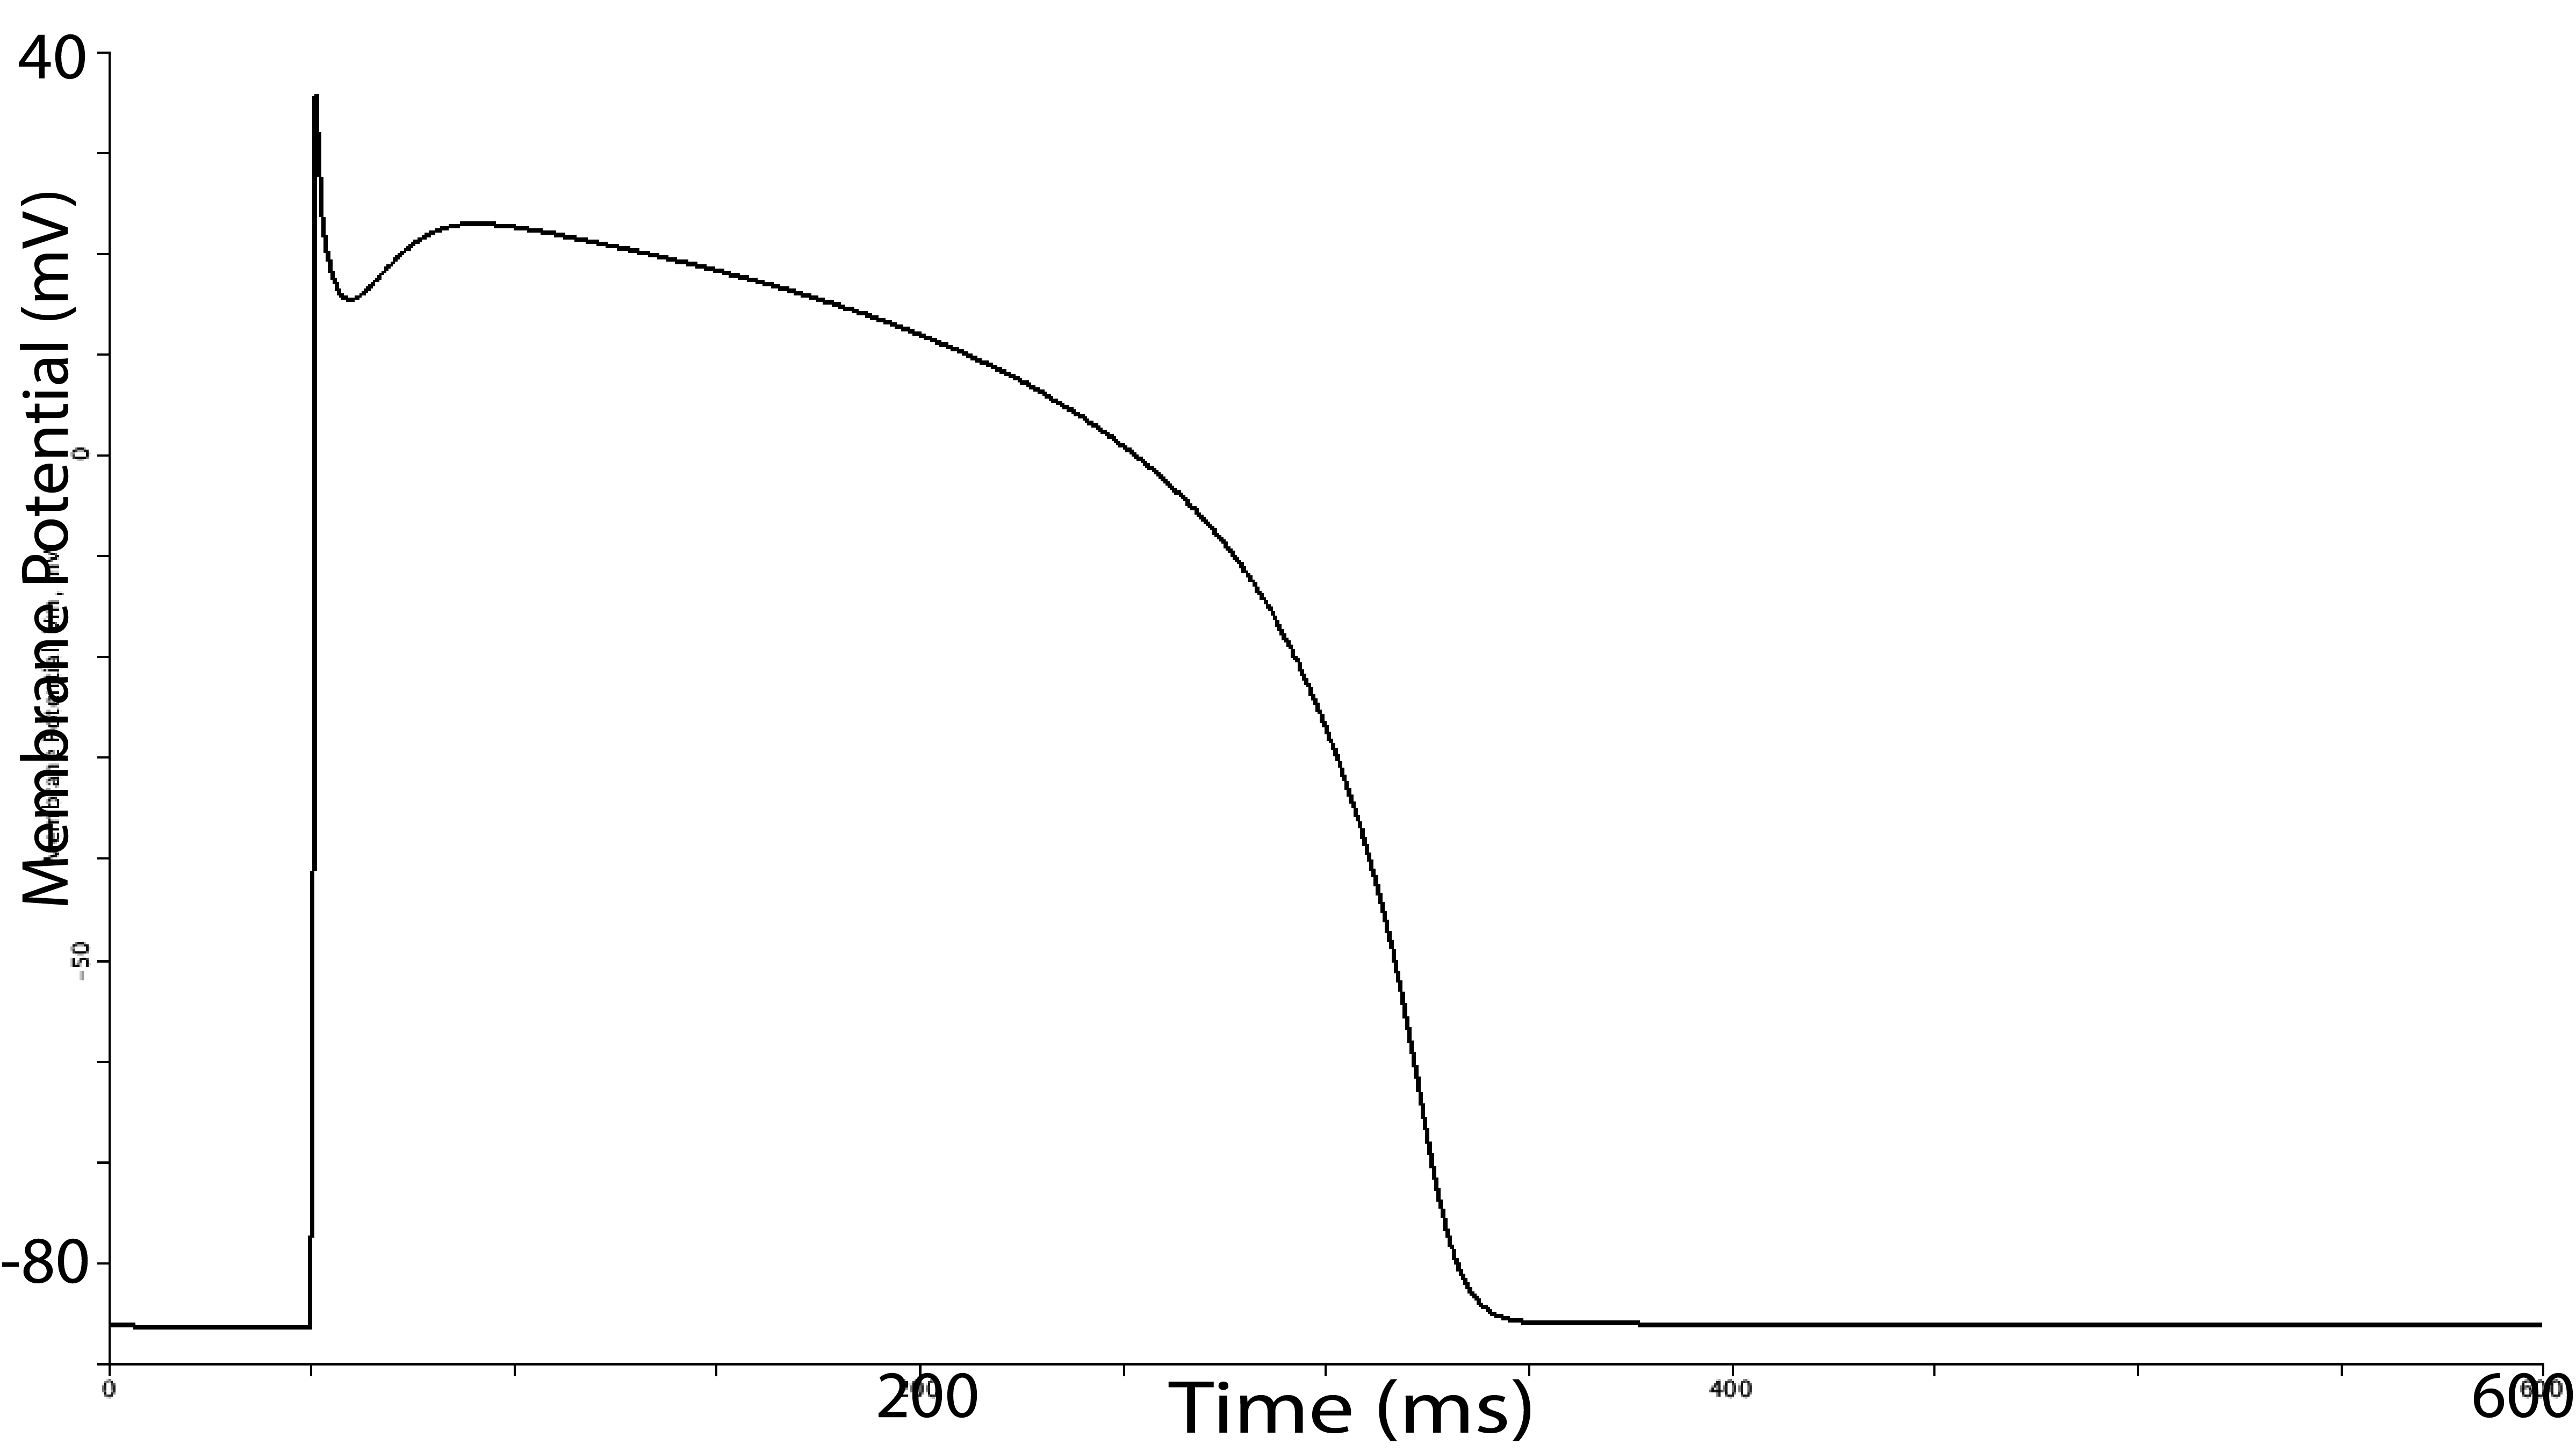
\includegraphics[width = \textwidth]{figs/originaleditK.png}
		\caption{}
		\label{exp1:c}
	\end{subfigure}
	\begin{subfigure}{0.45\textwidth}
		\centering
		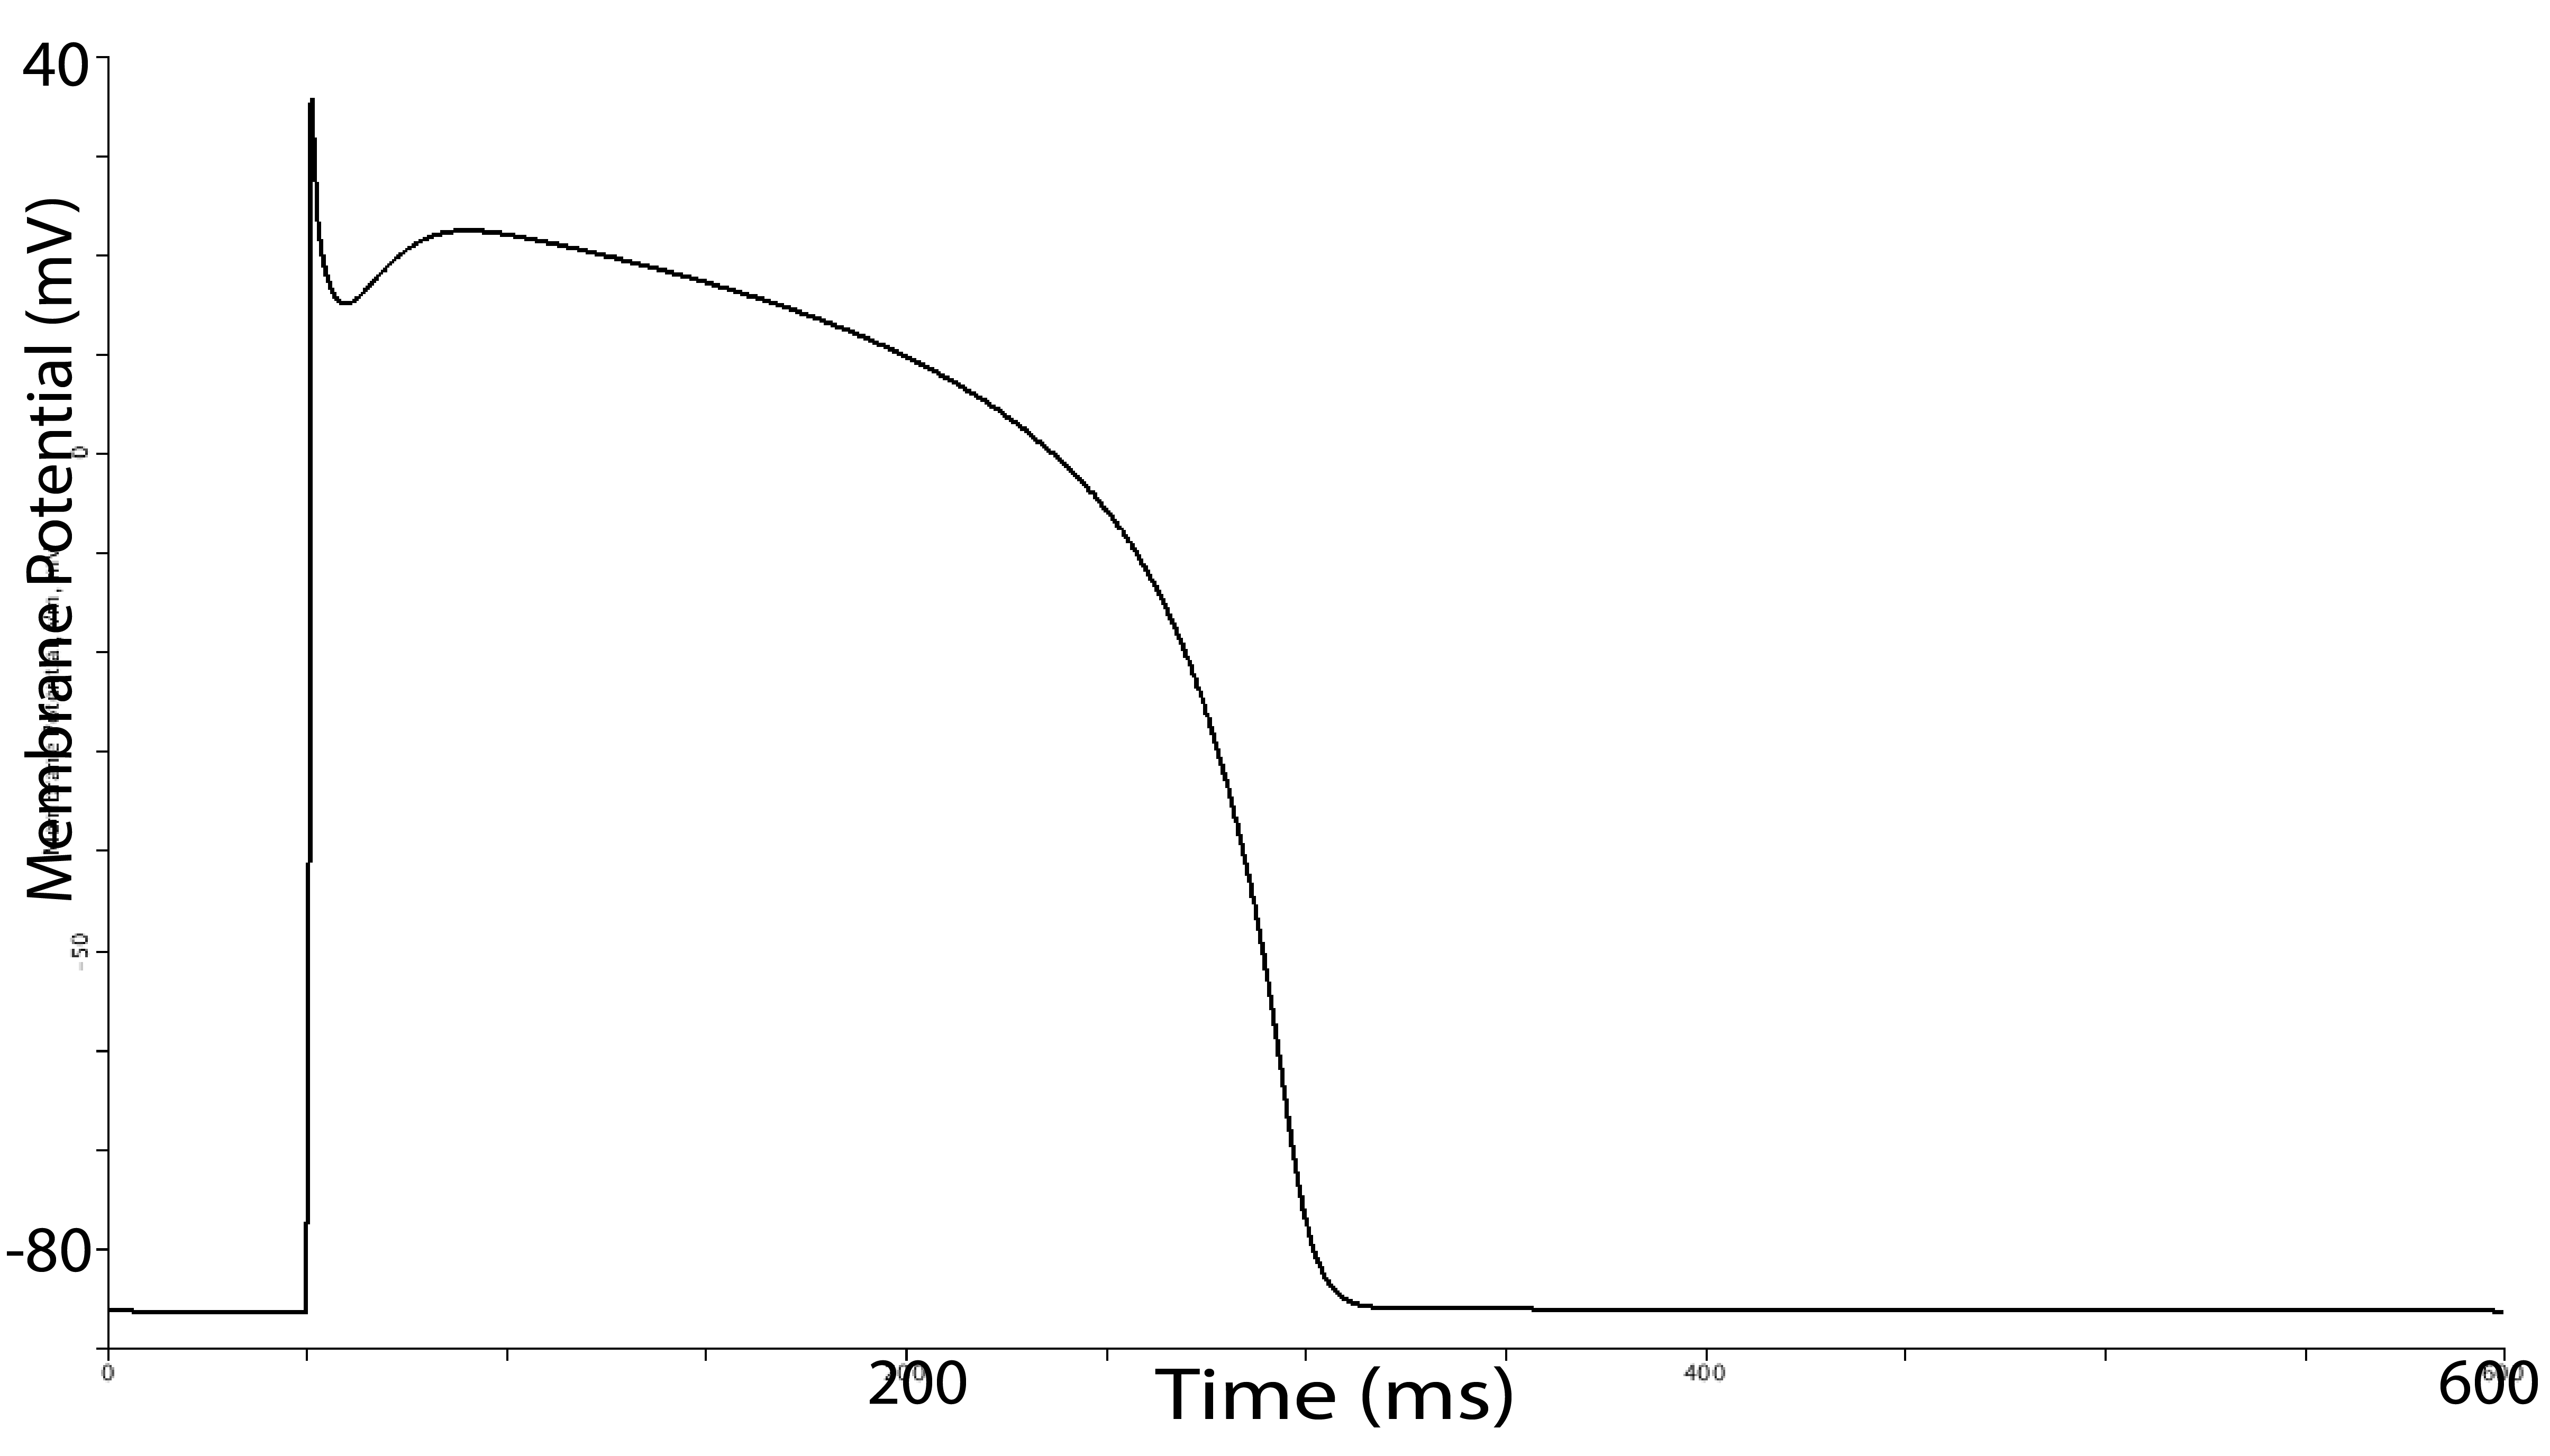
\includegraphics[width = \textwidth]{figs/200gkredit.png}
		\caption{}
		\label{exp1:d}
	\end{subfigure}
	\caption{Membrane potential at each conductance value for the hERG potassium channel after simulation. A: Conductance set to zero B. Conductance set to 50\% normal conductance, C: Conductance set to 100\% conductance, D: Conductance set to 200\% conductance. There is a marked decrease in action potential time with each increase in conductance. Units are in millivolts on the y axis and time (milliseconds) on the x axis}
	\label{fig:exp1}
\end{figure}
\par{}
To quantify this we calculated the APD90 time. This is the time it takes for the membrane to repolarize by 90\%, or reach a voltage that is 10\% of the peak voltage. The time of the beginning of the action potential (50 ms for our simulations) is then subtracted from these times to give us the APD90 time. These times are displayed in Table \ref{tab:potassium}. As can be seen, as conductance increases, ADP90 time decreases, as expected. Again this falls in line with our model as hERG contributes to repolarization. A lesser hERG conductance will result in a delayed reploarization, and therefore a higher APD90.

\rowcolors{2}{gray!25}{white}
\begin{table}[H]
	\centering
	\caption{Calculated APD90 times for each hERG channel conductance}
	\label{tab:potassium}
	\begin{tabular}{cc}
		\hline \hline
		hERG Conductance & APD90 (milliseconds)\\ 
		nanoseimens/picosecond &  \\
		\hline
		0\% Conductance & 318\\ 
		50\% Conductance &  297\\ 
		
		100\% Conductance &  278\\ 
		
		200\% Conductance&  249\\ 
		
		
		\hline 
		\hline
	\end{tabular} 
\end{table}
\par{}
These simulations can easily represent different physiological states for the hERG channel. In the case of lesser conductance, this could represent the effects of hERG blocker drugs or a mutated hERG channel that is less conductive to potassium. The increase hERG conductance tests can represent the effects of hERG activating drugs or activating mutations. In either case, the power of this simulation is that it allows for the exploration of these different situations. For example, suppose we have developed a drug that we want for treatment of a disease, but we learn through chemical analysis that it may affect the hERG conductance. We have three forms of the drug that change the hERG conductance by different amounts. By testing them in such a simulation as this we could investigate the effects of this drug on the cardiac action potential. Changes in the action potential such as those we see by varying the hERG conductance can have sever effects on cardiac health. Changes in repolarization time can lead to long or short QT syndrome, which are extensions or reductions iin the length of the qt segment of the ECG cause by longer or shorter repolarization/APD90 respectivly. Conditions such as these can often cause lead to arrhythmia and even sudden cardiac death. 

\subsection{Calcium conductance}
\par{}
During this section we tested the effects of adjusting the calcium conductance across the membrane and the effect on intracellular calcium concentration and recovery as well as time to peak concentration and APD90 of the action potential. In figure \ref{fig:exp1} we see the calcium concentration in the cytosol during the simulations. As can be seen the time to peak is delayed with each increase in conductance, while the rate of decay for the concentration decreases with each increase in conductance. Given our understanding of the model this makes sense. As calcium is released from the SR the intracellular calcium increases in concentration. With increased calcium conductance at the membrane this intracellular calcium can simultaneously flow out of the cell. Thus the time it takes to reach the peak calcium is delayed with increased conductances as calcium is flowing out faster. The time constants also decrease with each increase in conductance. At first this can seem counter intuitive. However when we consider that the increased conductances result in a higher peak, and thus a longer time to recover. Additionally the time constants should increase because as we are pumping calcium back out of the cytoplasm, the increased conductance continues to allow it to flow into the cytoplasm, thereby decrease the rate fo recovery and increasing the time constant. Overall we would expect this to have an effect of lengthening the duration of the action potential, as it takes longer for the cell to get rid of the calcium in each increased conductance case. Thus the cell will remain positive for longer.
\begin{figure}[H]
	\centering
	\begin{subfigure}{0.45\textwidth}
		\centering
		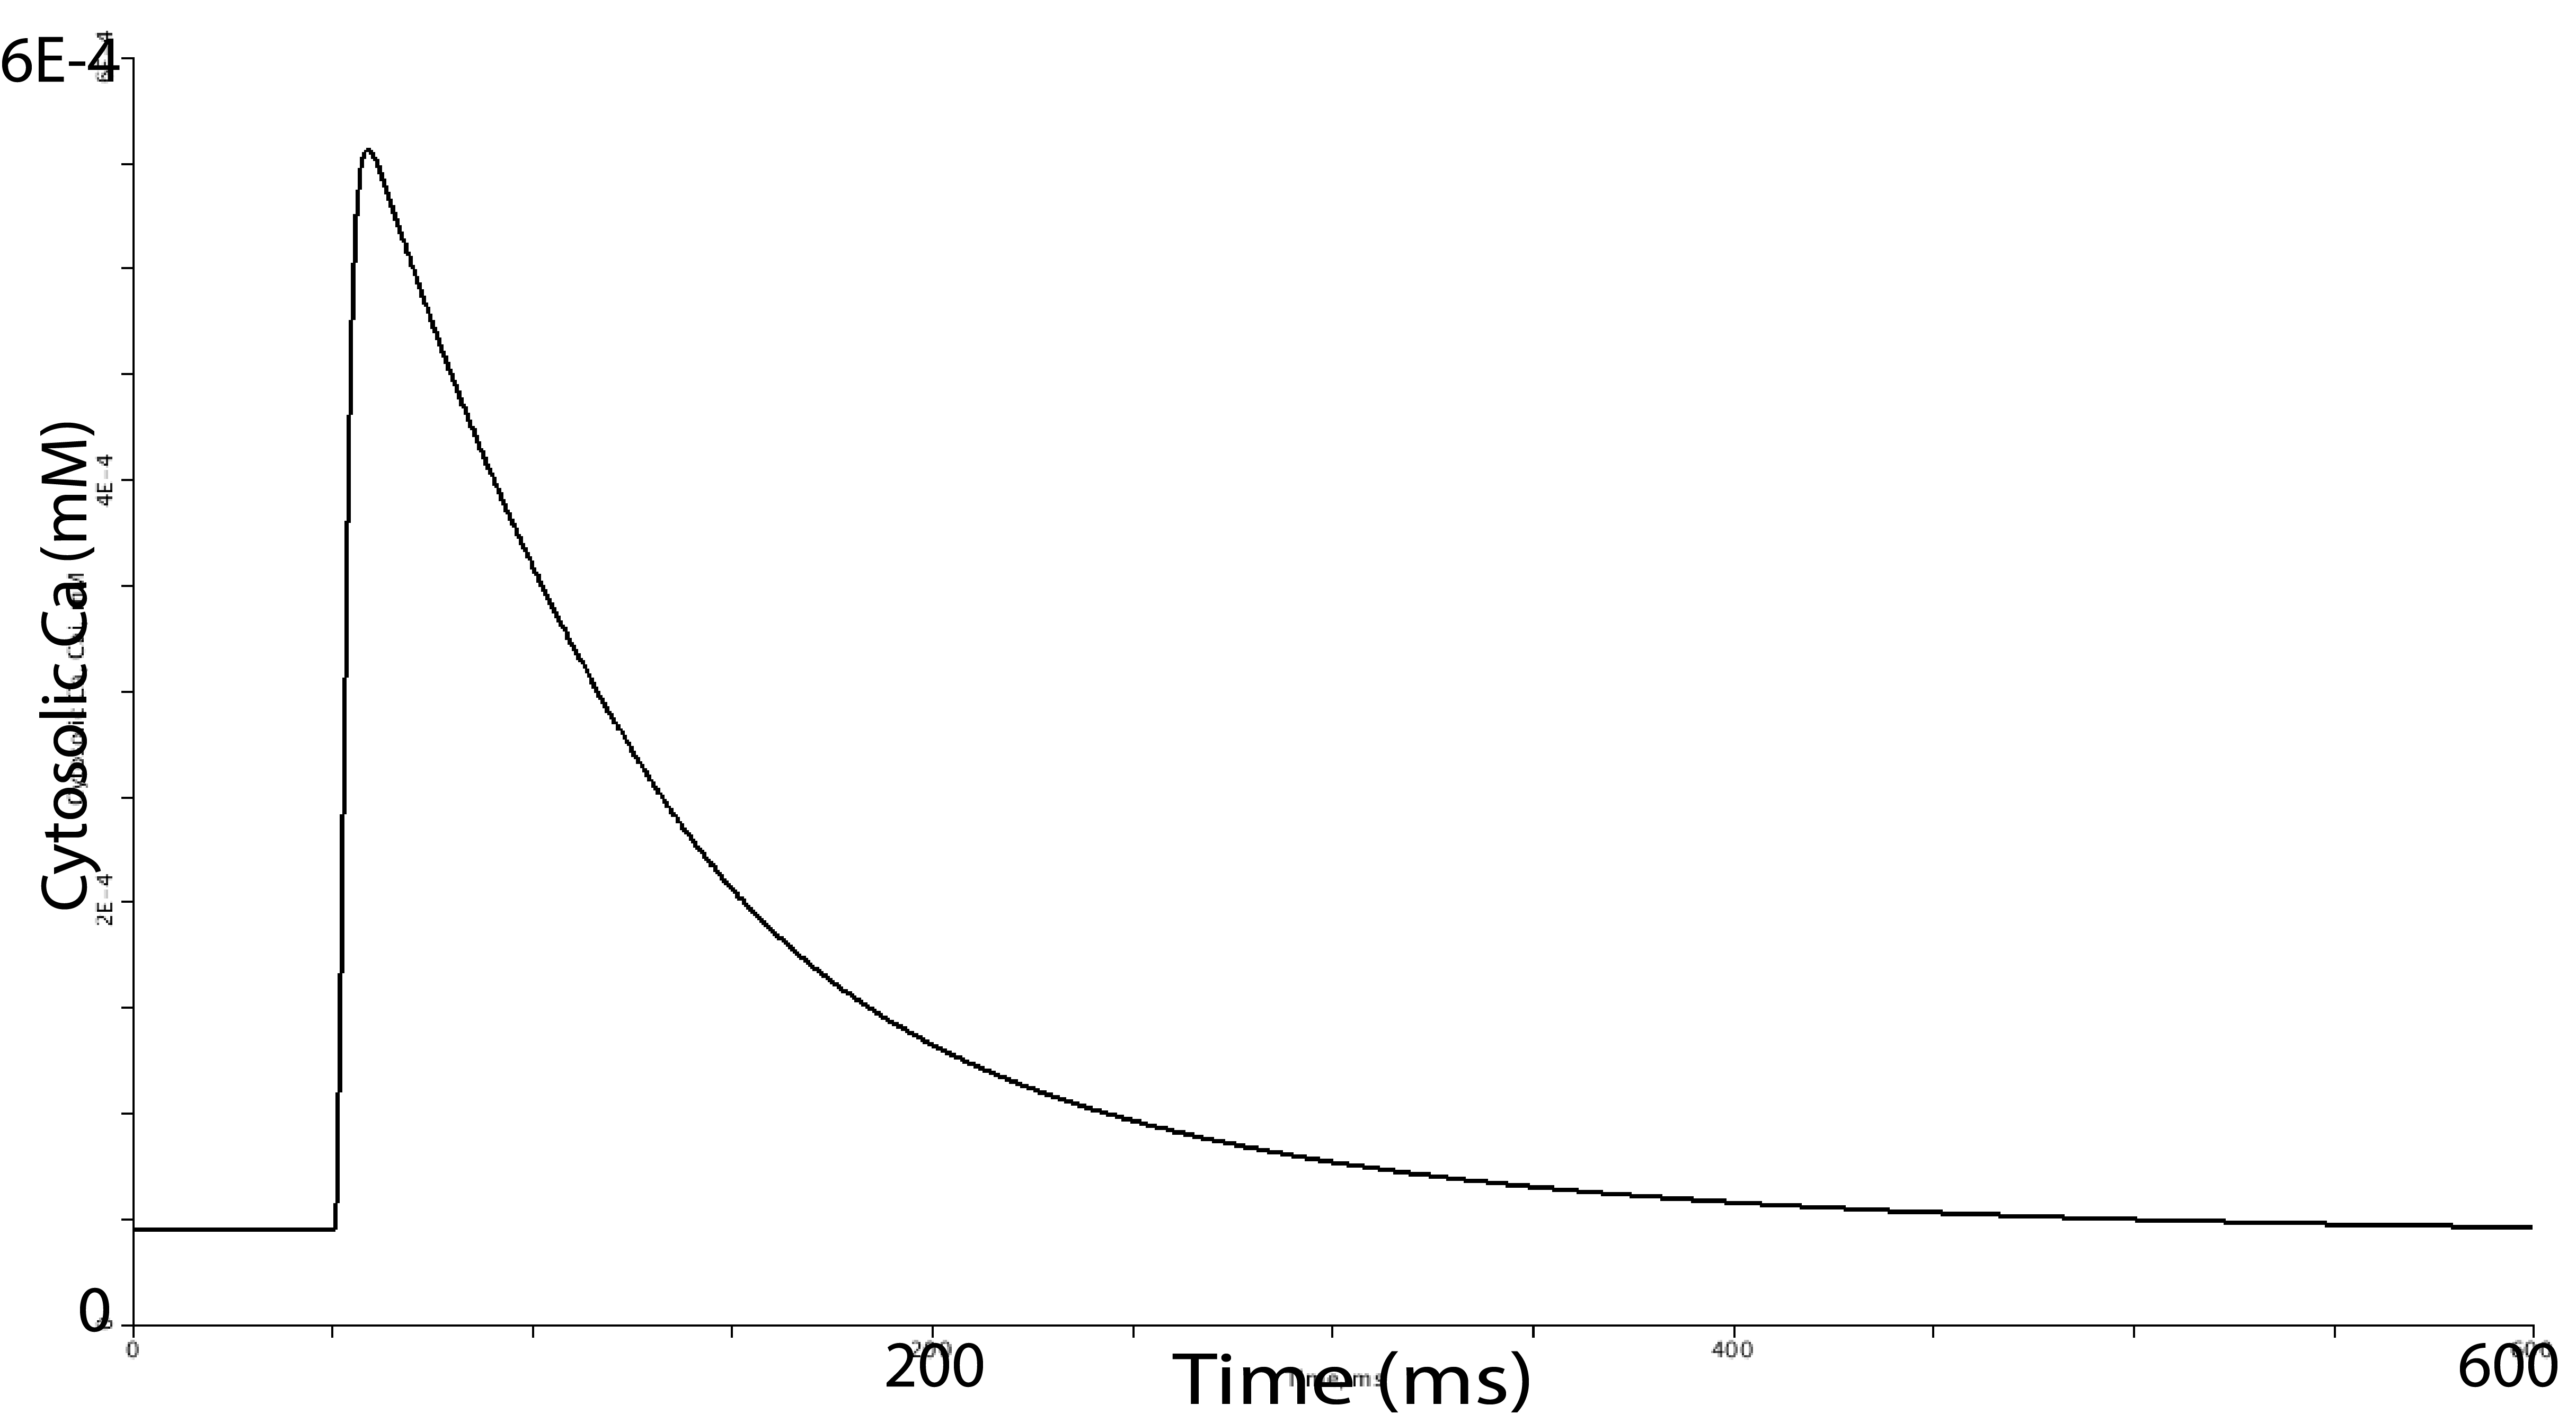
\includegraphics[width = \textwidth]{figs/0gcaledit.png}
		\caption{}
		\label{fig:left}
	\end{subfigure}
	\begin{subfigure}{0.45\textwidth}
		\centering
		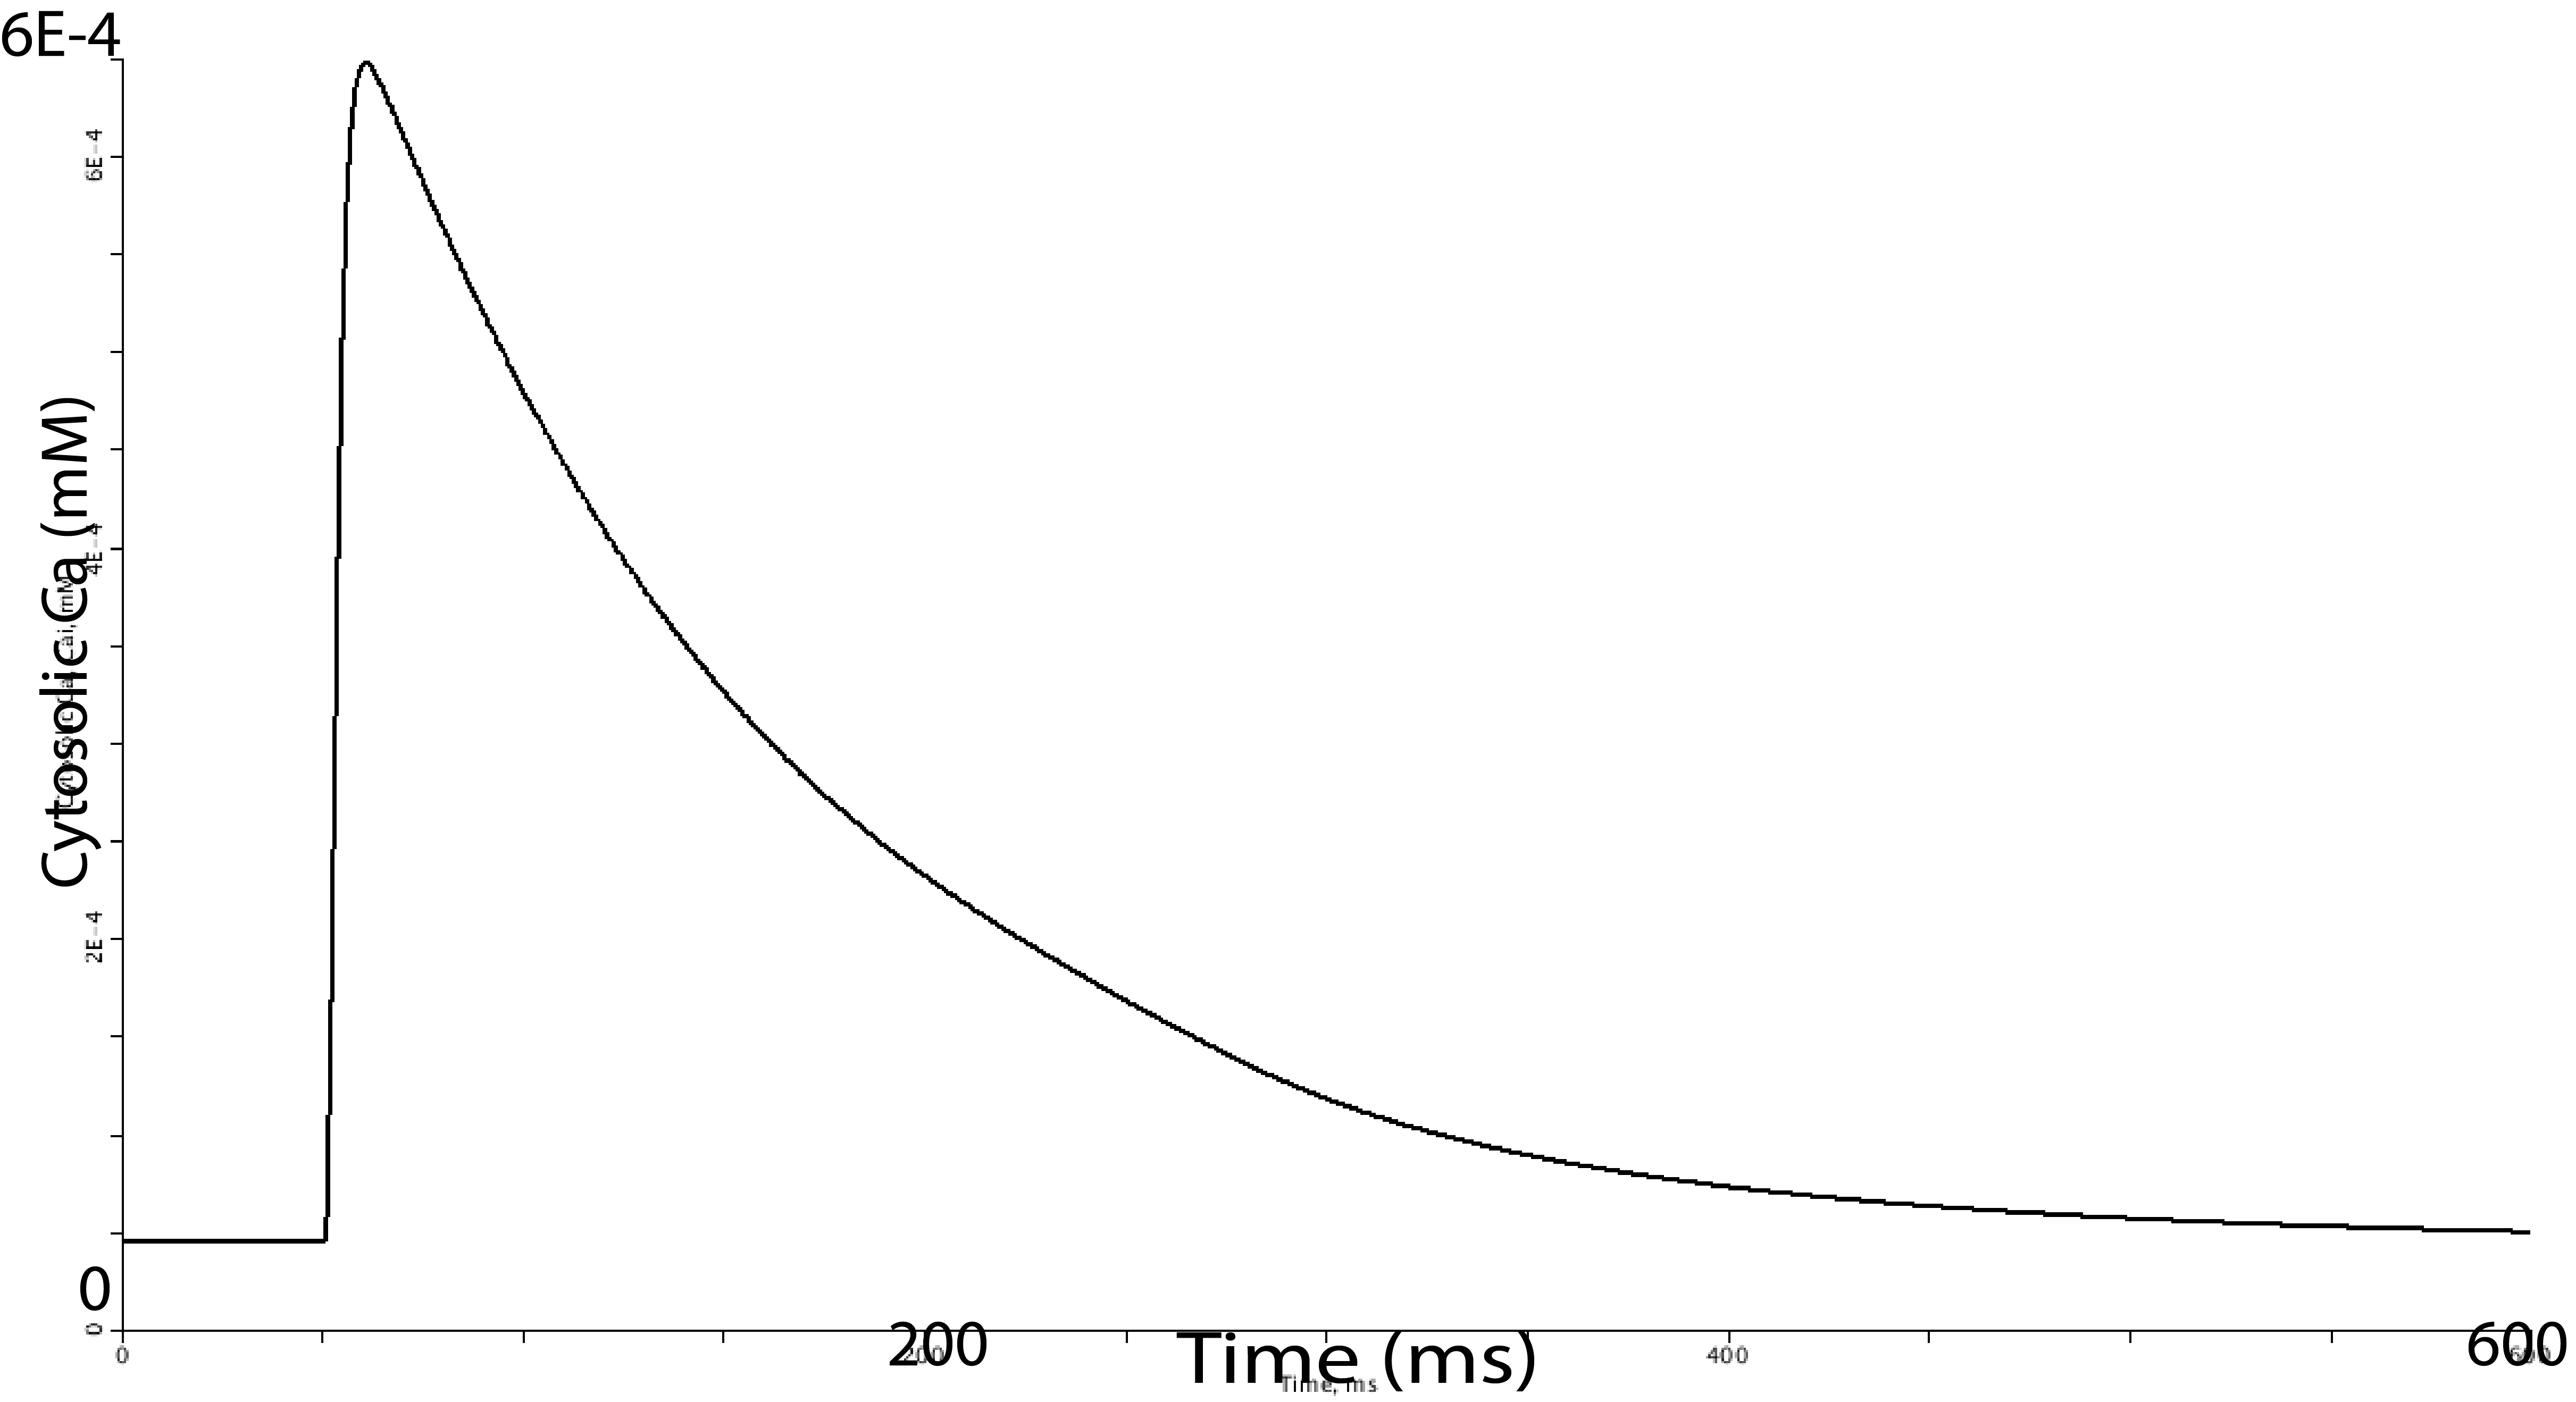
\includegraphics[width = \textwidth]{figs/50gcaledit.png}
		\caption{}
		\label{fig:right}
	\end{subfigure}
	\vskip\baselineskip
	\begin{subfigure}{0.45\textwidth}
		\centering
		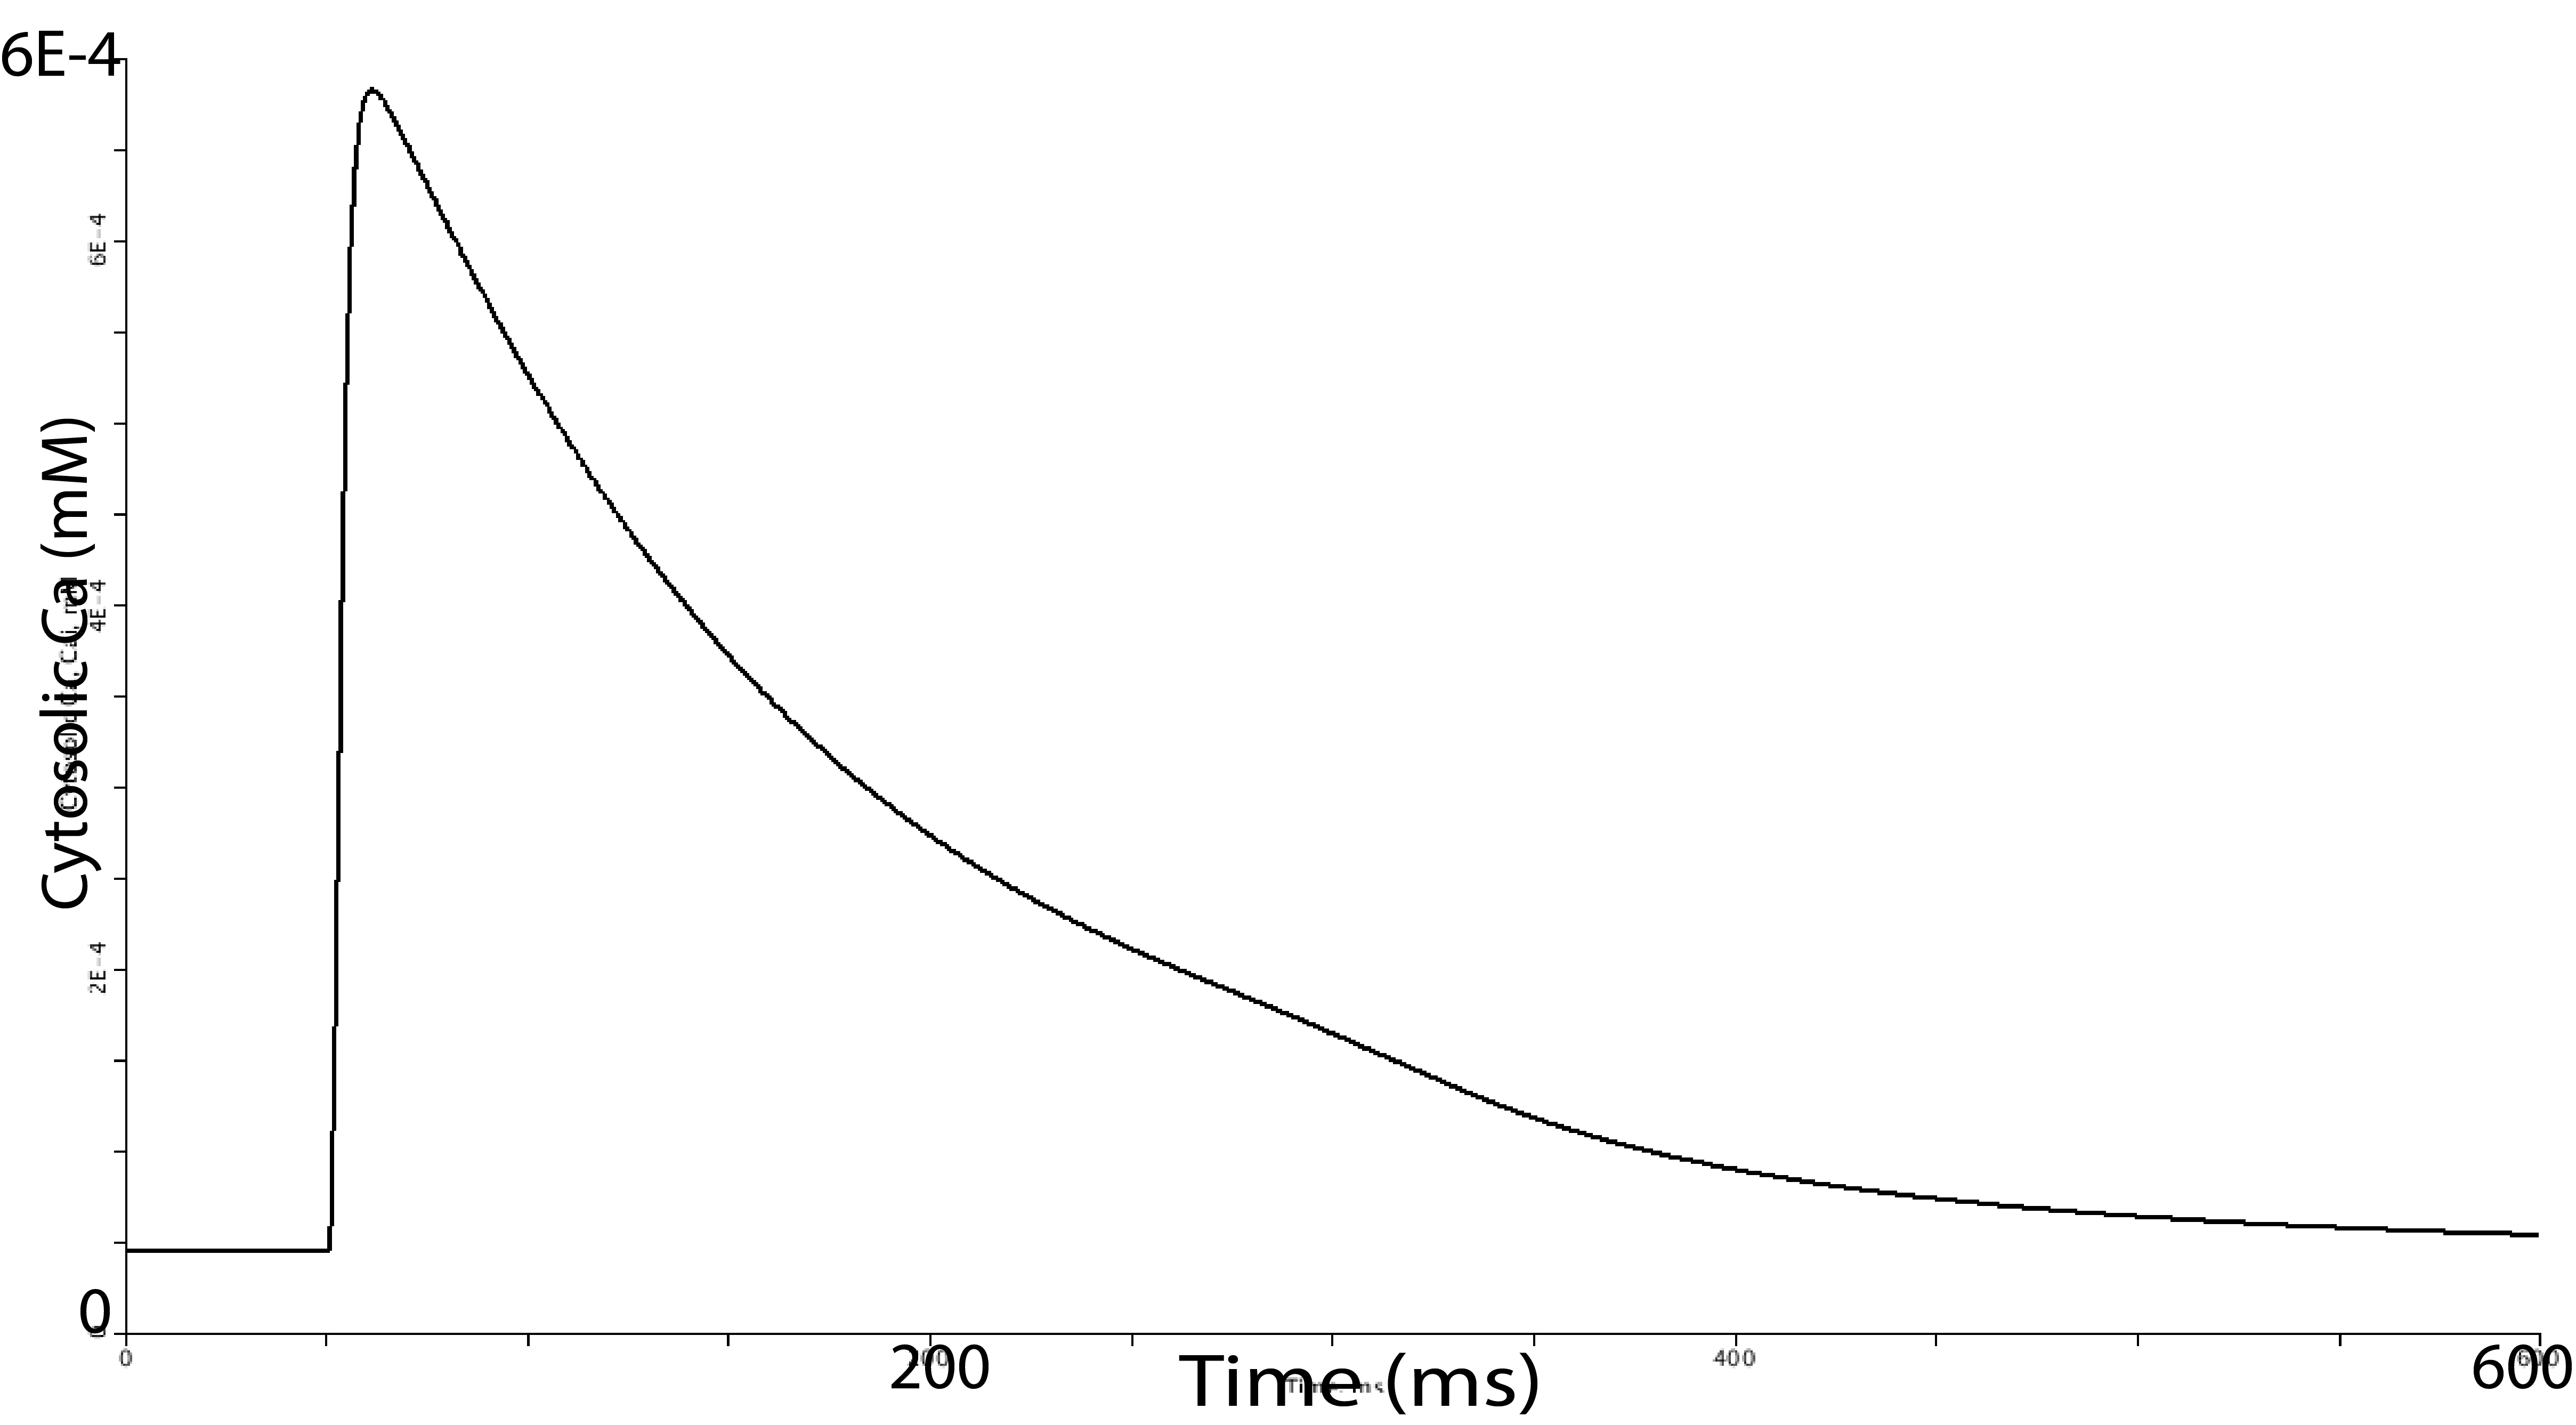
\includegraphics[width = \textwidth]{figs/originaleditCa.png}
		\caption{}
		\label{fig:left}
	\end{subfigure}
	\begin{subfigure}{0.45\textwidth}
		\centering
		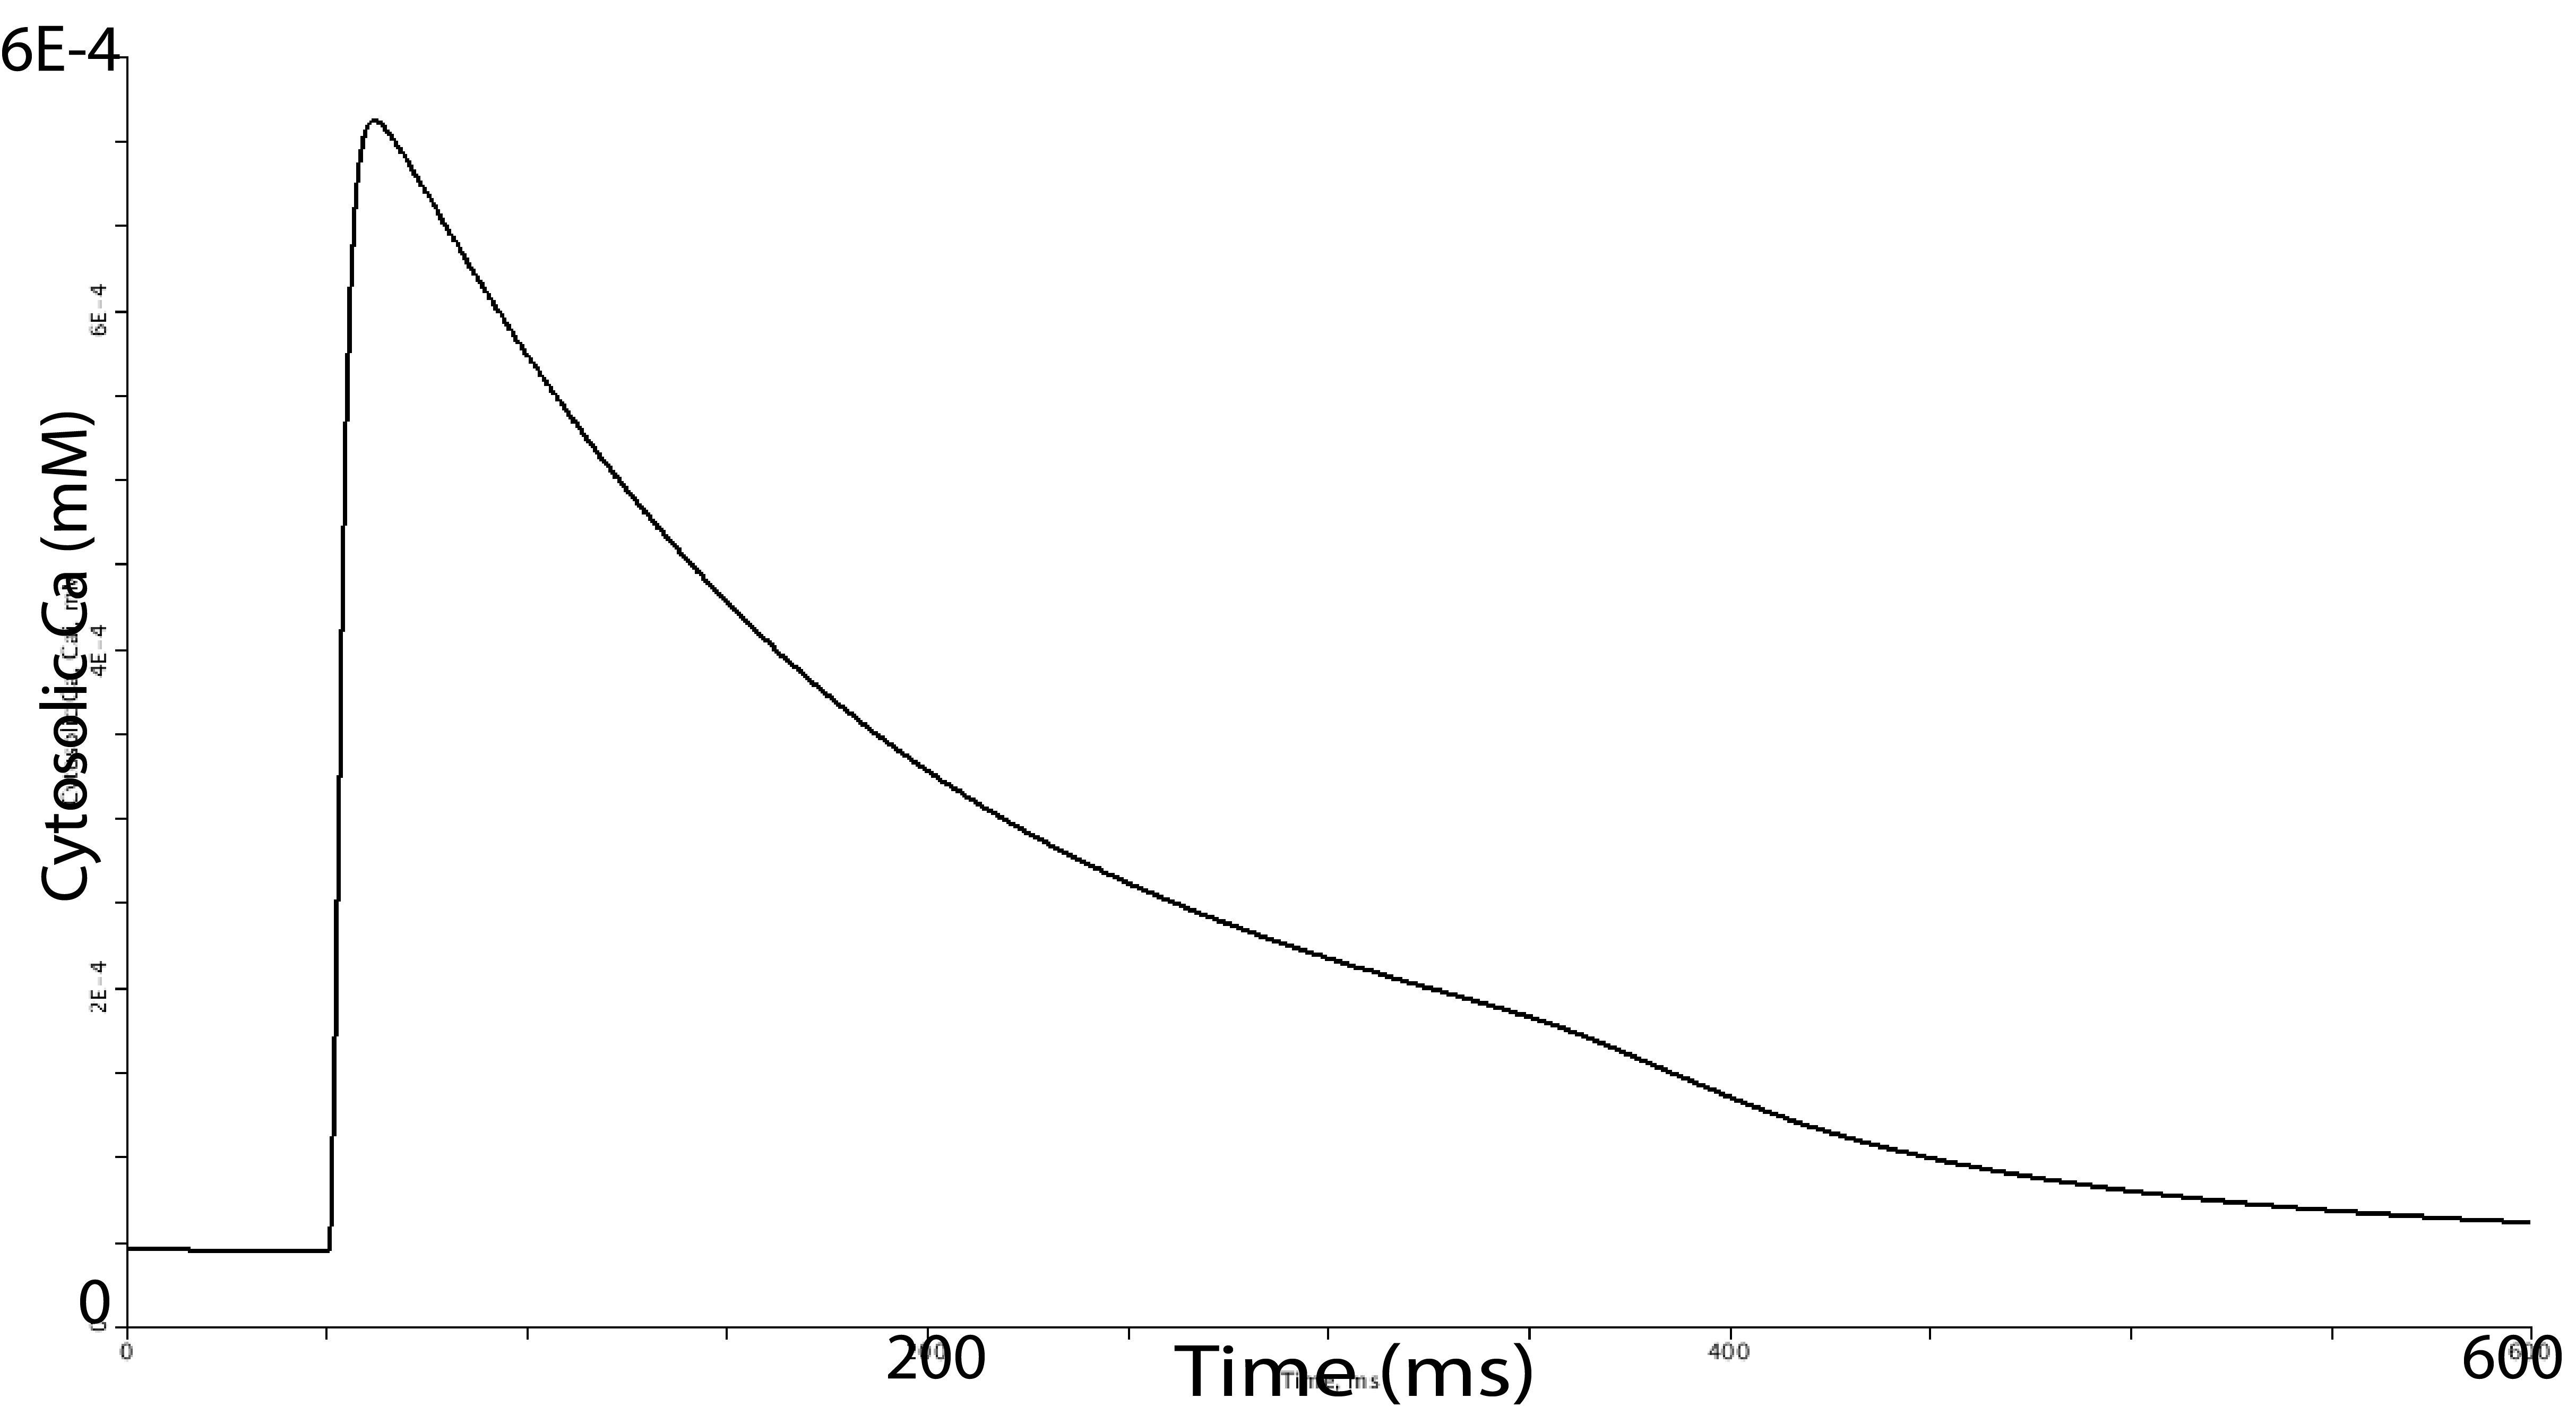
\includegraphics[width = \textwidth]{figs/200gcaledit.png}
		\caption{}
		\label{fig:right}
	\end{subfigure}
	\caption{Intracellular calcium concentration for each G\_Cal conductance. A: Conductance set to zero B. Conductance set to 50\% normal conductance, C: Conductance set to 100\% conductance, D: Conductance set to 200\% conductance. The time constant appears to be reduced with each conductance increase. Units on the graph are in concentration (millimolar) on the y axis and time (milliseconds) on the x axis}
	\label{fig:exp2}
\end{figure}

\par{}
When we observe the metrics measured in Table \ref{tab:calcium} we see that the ADP90 and time to peak follow our predictions, but the time constants do not. However when we consider the fits that excel provided in Figure \ref{fig:original} it becomes more clear why this might be the case. During our model there was a strange inflection during the recovery that may ahve been difficult for excel to model. Additionally the 0 \% conductance in figure \ref{fig:overlays} a seems to have a very poor fit for some reason, reflected in its poor R squared value of 0.858. However if we consider what we see in figure \ref{fig:exp2} we can clearly see that the decay is less in each increase in conductance, in accordance with our predictions and reasoning.
\par{}
Modulating these calcium conductances will not only affect the action potentials of a cardiomyocyte but also the contraction via excitation-contraction coupling. The initiation of the action potential results in the release of calcium which triggers the cascade leading to contraction of the actin-myosin filaments in the cell. By modulating the calcium conductance we affect this process. A delay in caclium peak would cause a delay in contraction, while a delay in the recovery of calcium would cause an extended contraction. Taken together these could lead to detrimental affects on the propagation and coordination of contraction in the hear.
\par{}
This model does not seem to display much information relating to this excitation contraction coupling. To improve this I would add terms to the model that determine contraction strength, initiation, and duration, dependent on the calcium concentration. Additionally contraction and stretch of the myocyte affect other conductances which could be incorporated to better represent the activities of such a myocyte.


\rowcolors{2}{gray!25}{white}
\begin{table}[H]
	\centering
	\caption{Calculated APD90, Time to Peak (TTP), and Time constants for calcium transients resulting from the shown changes in the calcium channel conductance (g\_Cal)}
	\label{tab:calcium}
	\begin{tabular}{ccccc}
		\hline \hline
		Calcium Conductance & APD90  & Time To Peak  & Time Constant & R-squared\\ 
		L/(faradsSeconds) & (milliseconds) & (milliseconds)& (milliseconds)& \\
		\hline
		0\% Conductance & 74& 5.95&240 &0.858 \\ 
		50\% Conductance &222 &7.55 &204 &0.946 \\ 
		
		100\% Conductance & 278 &8.05 & 202& 0.977\\ 
		
		200\% Conductance& 344 & 8.70& 213& 0.995\\ 
		
		
		\hline 
		\hline
	\end{tabular} 
\end{table}

\begin{figure}[H]
	\centering
	\begin{subfigure}{0.45\textwidth}
		\centering
		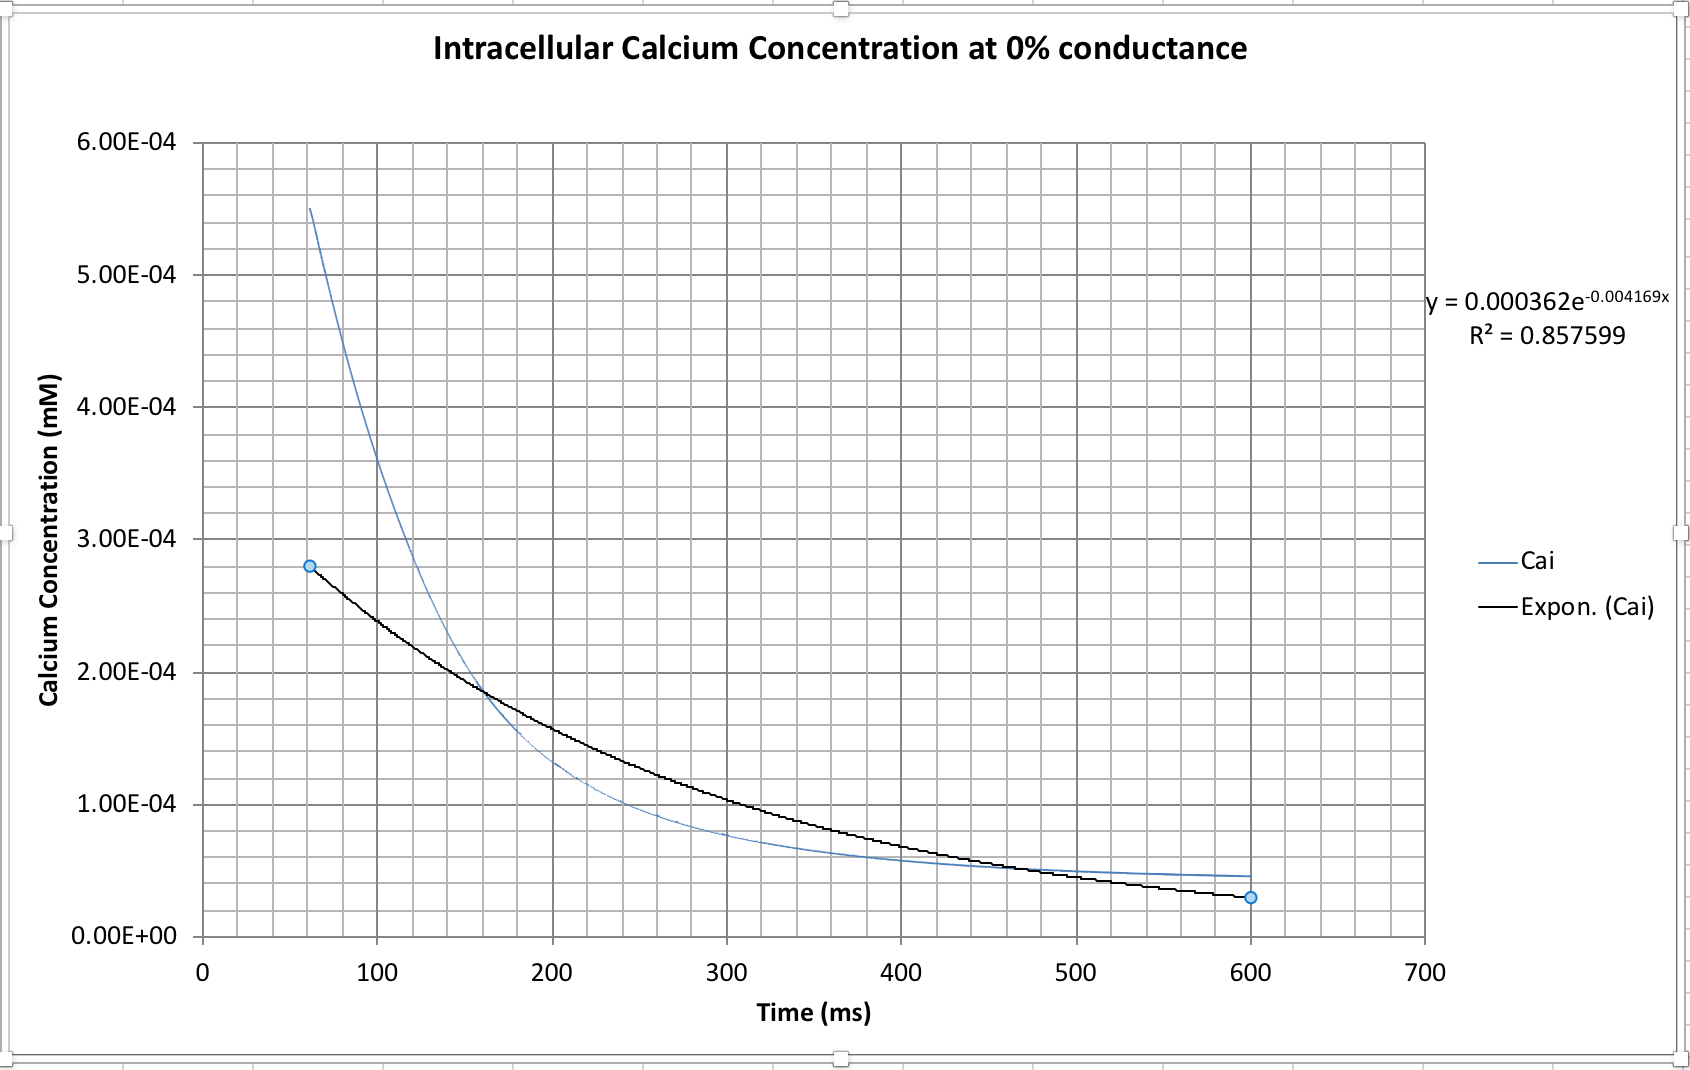
\includegraphics[width = \textwidth]{figs/3.png}
		\caption{}
		\label{fig:left}
	\end{subfigure}
	\begin{subfigure}{0.45\textwidth}
		\centering
		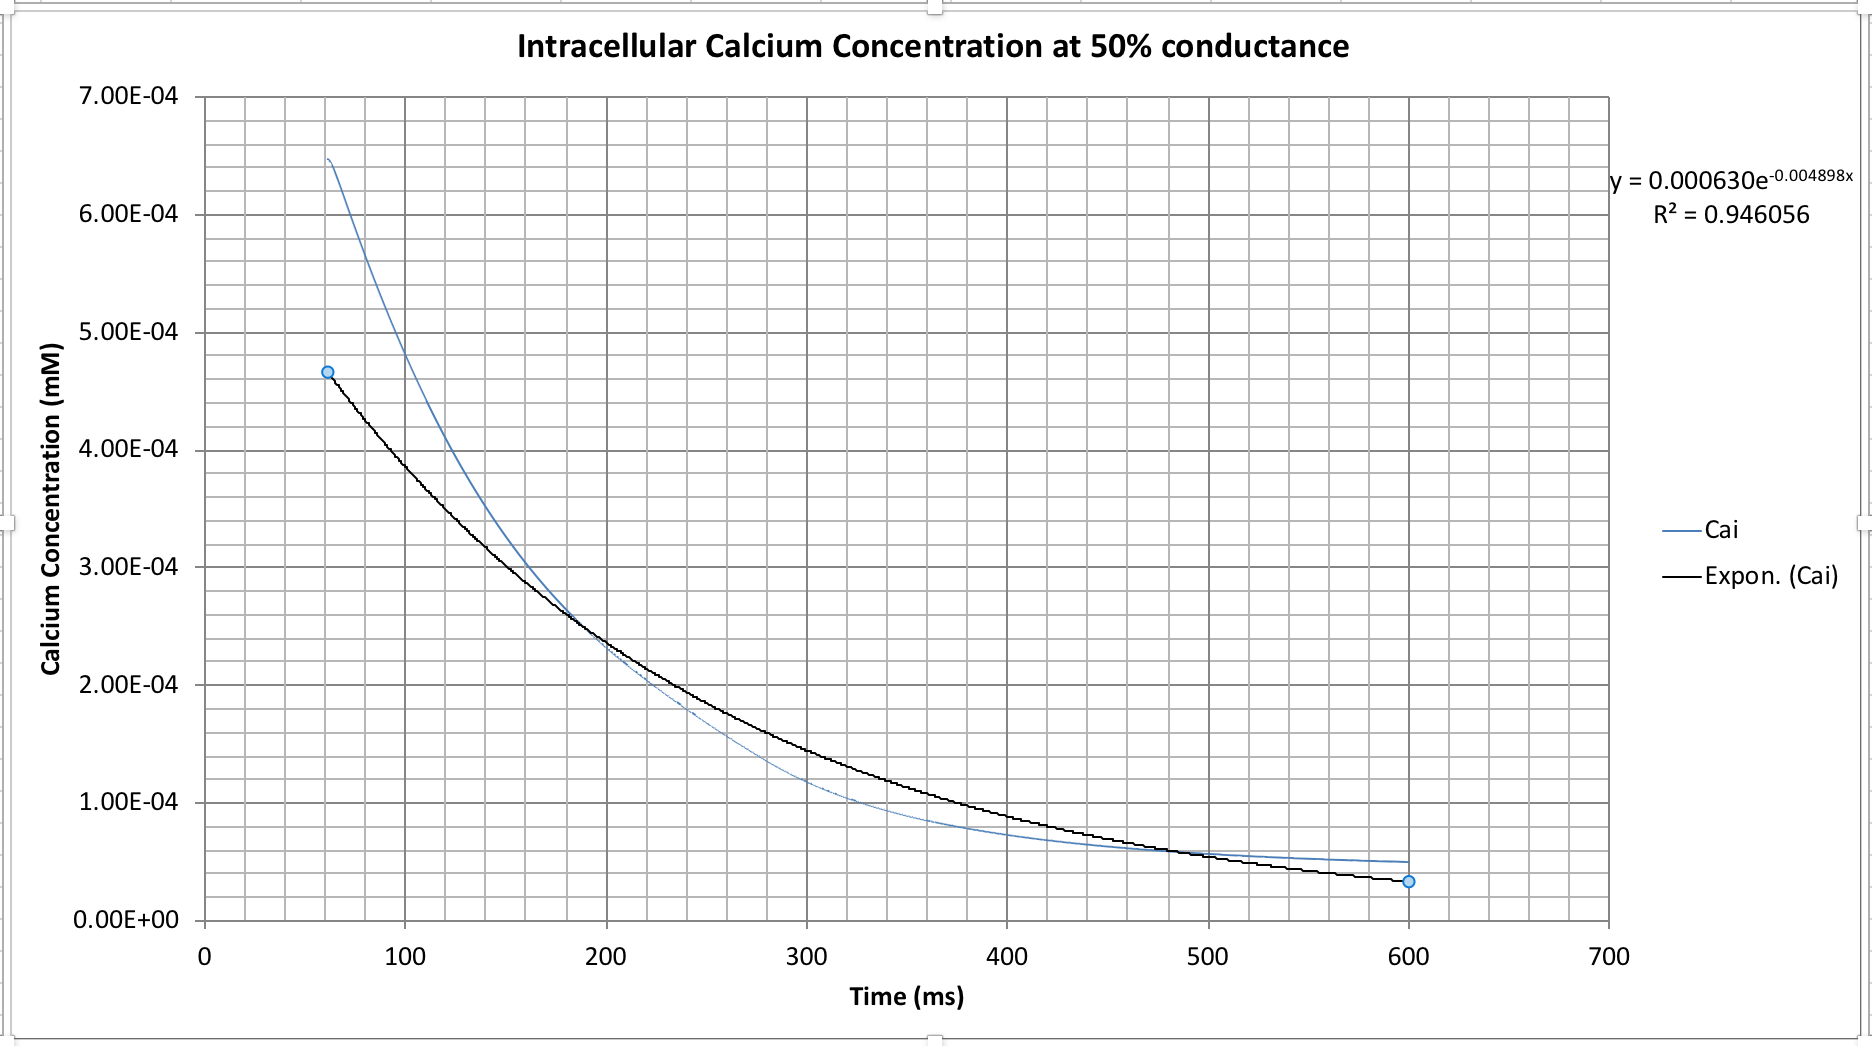
\includegraphics[width = \textwidth]{figs/2.png}
		\caption{}
		\label{fig:right}
	\end{subfigure}
	\vskip\baselineskip
	\begin{subfigure}{0.45\textwidth}
		\centering
		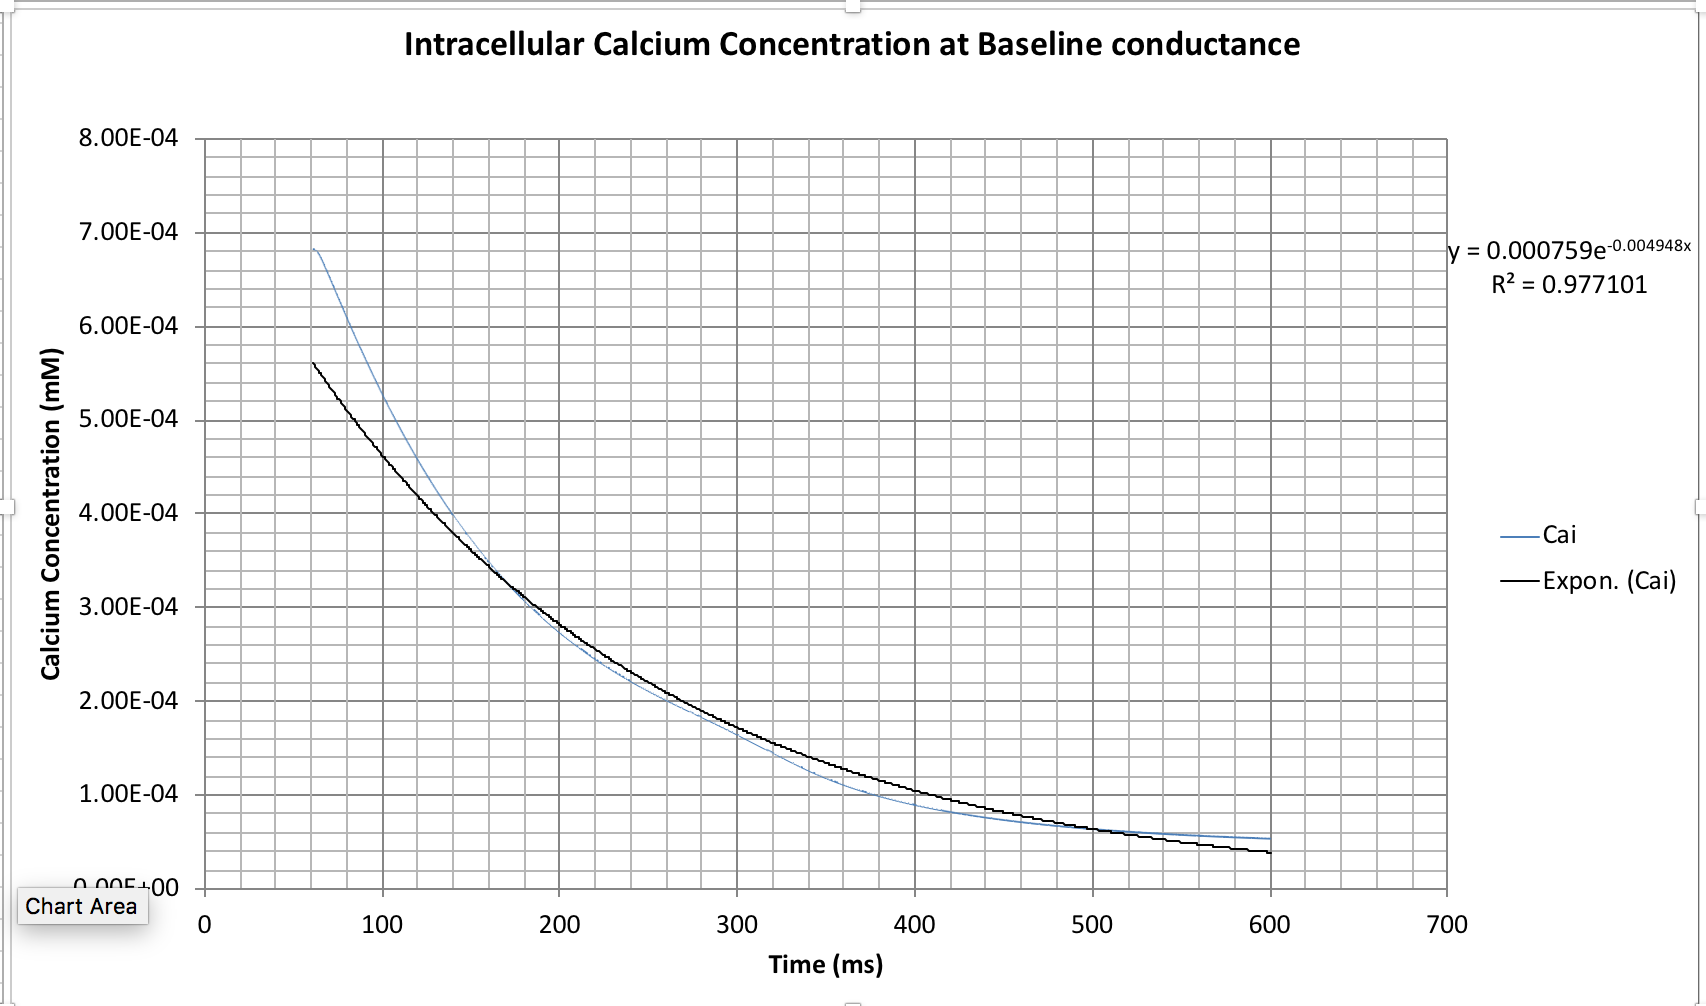
\includegraphics[width = \textwidth]{figs/1.png}
		\caption{}
		\label{fig:left}
	\end{subfigure}
	\begin{subfigure}{0.45\textwidth}
		\centering
		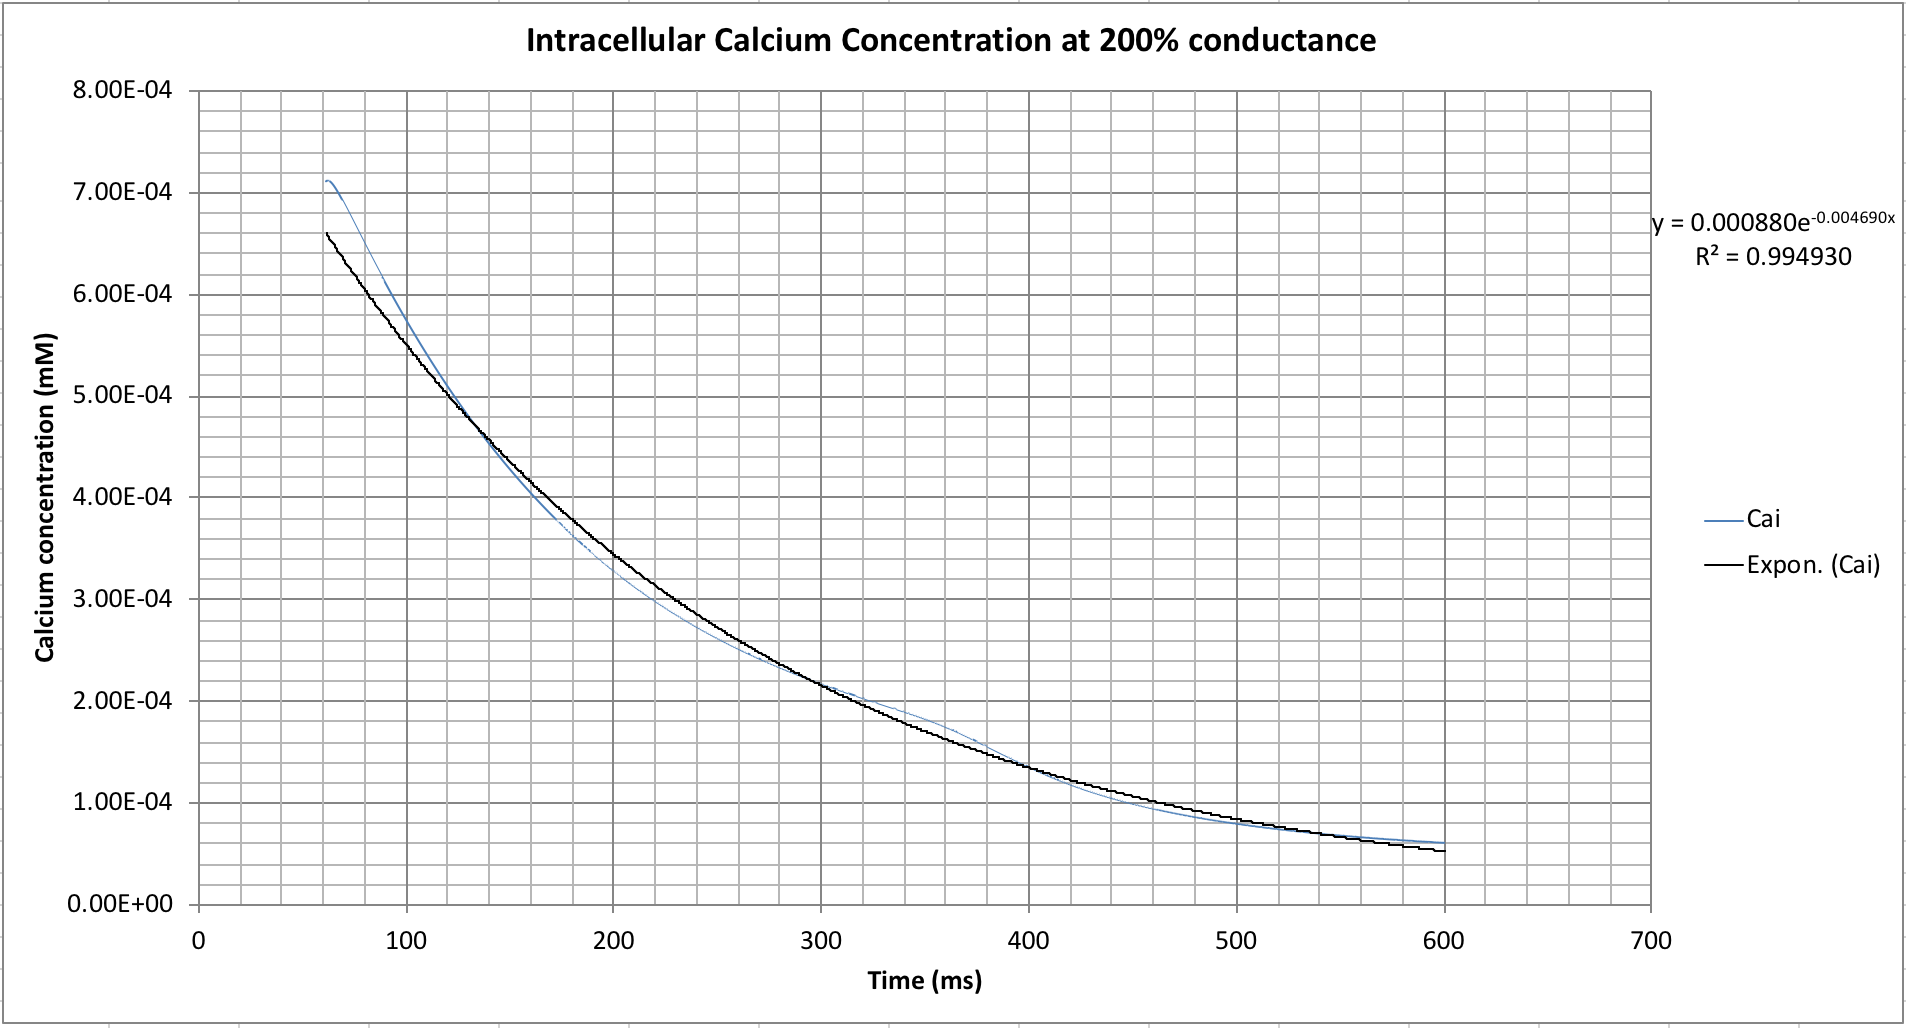
\includegraphics[width = \textwidth]{figs/4.png}
		\caption{}
		\label{fig:right}
	\end{subfigure}
	\caption{Summary figure of the intracellular calcium Decay with overlay concentration based on changes to the calcium conductance. A. Zero Conductance B. 50\% normal conductance, C. 100\% conductance, D. 200\% conductance. Units on the graph are in concentration (millimolar) on the y axis and time (milliseconds) on the x axis}
	\label{fig:overlays}
\end{figure}


\section{Conclusion}
The purpose of this lab was to build upon our knowledge of cardiac cell modeling, and cellular modeling in general. We explored the use of the Ten Tusscher\cite{TenTusscher2003} model to simulate the effects of changing potassium and calcium conductance on the behavior of the cell, and contemplate the ramifications of these effects. This lab allowed us to explore the versatility of the JSim modeling environment and the ease at which we are able to use it to perform hypothesis testing on these modeled cells. Traditional cardiac cell models only incorporate potassium, sodium, and leak currents into their formulation. However the model we used today incorporated a calcium conductance, which we know from experimentation to be an important part of cardiac electro physiology. This improvement over the traditional models where calcium conductance is lumped into the leak conductance proved vital for a more in depth understanding of a cardiac model. In particular, without considering the calcium conductance we would not be able to discuss the principles of excitation-contraction coupling. This model allowed us to investigate the profound effect that calcium conductances can have on the action potential, as seen in Table \ref{tab:calcium} where the APD90 was severely effected by the calcium conductance changes.
\par{}
Without the use of this computational model, an experiment such as this would take moths or even years when considering the time it would take to culture cells, gain the technical training necessary, and perform enough successful experiments to generate enough usable data. This does not even include the enormous cost of such an endeavor. However, via the use of this computational model, we were able to perform these investigations repeatedly, quickly, and with only the use of a personal computer. Even a laptop has enough computational power to perform these modeling calculations. Thus we are able to easily change parameters and receive near instant results. Thus we can rapidly iterate through many different parameter sets and scenarios, allowing for a robust exploration of the model.
\par{}
These computational advances are however not without drawbacks. Computational models are limited in scope and their limitations must be considered whenever using them. This particular model does not seem to model the effects of excitation-contraction coupling or any other mechanical properties of the cell. Thus all questions posed of this model must be within the framework set out by the model.
\par{}
Overall we utilized this model to gain a better understanding of the effects of the hERG potassium conductance and the calcium conductance on the action potential and the intracellular calcium concentration. Due to the robust and light weight nature of this model we are able to rapidly and precisely change the parameter values iteratively and rapidly assess the results. The JSim software allows an integrated inputs and outputs workspace where the model can be interactively modified and explored. Overall this lab expanded our understanding both of the specifics of cardiac myocytes in respect to the discussed conductances but also the principles of cell modeling.



%%%%%%%%%%%%%%%%%% Correct Bibliography Style

\bibliography{C:/Users/Jake/Documents/library}
\bibliographystyle{IEEEtran}


\section{Appendix} 
Matlab Code Used:\newline
\%Data loaded in from JSIM\newline
data = table2array(calData(:,1)); \newline
calcConcentration = table2array(calData(:,3));\newline
[peakValuePrime, peakTimePrime] = max(diff(calcConcentration));\%location of upstroke\newline
[peakValue, peakTime] = max(Ca);\%location of peak\newline
TimeToPeak = data(pealValuePrime) - data(peakValue); \newline
\newline
actData = table2array(apData(:,1));
actPot = table2array(apData(:,3));
vB = actPot(1);\%The first value is the baseline value\newline
[vP,mxIdx] = max(actPot(:));\%Max value/peak value\newline
vAPD90 = vB + 0.1(vP-vB)\newline
APD90Time = 0;\newline
foundAPD90 = 0;
for idx = mxIdx:length(actPot)\newline
if and(actPot(idx) < vAPD90,foundAPD90 == 0)\newline
APD90Time = idx;\newline
foundAPD90 = 1;\newline
end\newline
end\newline

\end{document}


%%%%%%%%%%%%%%%% Table Example %%%%%%%%%%%%%%%%%%%%%%
\rowcolors{2}{gray!25}{white}
\begin{table}[H]
	\centering
	\caption{Simulated measurements for conduction velocity and maximal upstroke velocity}
	\label{tab:results}
\begin{tabular}{ccc}
	\hline \hline
	Experiment  & Conduction Velocity & Maximal Upstroke Velocity\\ 
	Number & (cm/ms)& (mV/ms) \\
	\hline
	 1 & 16.6389 &  69.8933 \\ 
	 2 &  18.9606&  73.9121 \\ 

	 3 &  24.7062&  83.871 \\ 

	  4&  45.2948&  109.1537\\ 

	  5&  52.6004&  116.8785\\ 

	  6&  77.6482&  131.6630\\ 

	  7&  2.0641&  0.0222\\ 

	  8&  44.0706&  109.3527\\ 

	  9&  45.2948&  109.1675\\ 

	  10&  2.1013&  -0.0024\\ 

	  11&  2.0896&  -0.0024\\ 

	  12&  60.3930&  179.3235\\ 
	  13&  38.8214&  86.8933 \\ 

	  14&  31.9728&  60.6956\\ 

	  15&  27.6375&  48.7076\\ 
	  16&  23.2945&  35.4873\\ 
	  17&  20.3827&  28.0958\\ 
	\hline 
	\hline
\end{tabular} 
\end{table}

%%%%%%%%%%%%%%%%% Figure Example %%%%%%%%%%%%%%%%%%%
	\begin{figure}[H]
	\centering
	\begin{subfigure}{0.49\textwidth}
		\centering
		\includegraphics[width = \textwidth]{../Simulation/Experiment_11.png}
		\caption{}
		\label{fig:left}
	\end{subfigure}
	\begin{subfigure}{0.49\textwidth}
		\centering
		\includegraphics[width = \textwidth]{../Simulation/Experiment_9.png}
		\caption{}
		\label{fig:right}
	\end{subfigure}
	\vskip\baselineskip
	\begin{subfigure}{0.49\textwidth}
		\centering
		\includegraphics[width = \textwidth]{../Simulation/Experiment_4.png}
		\caption{}
		\label{fig:left}
	\end{subfigure}
	\begin{subfigure}{0.49\textwidth}
		\centering
		\includegraphics[width = \textwidth]{stimulation.png}
		\caption{}
		\label{fig:right}
	\end{subfigure}
	\caption{Changes in Stimulation Current. (a) Output figure from experiment 11. (b) Output figure from experiment 9. (c) Output figure from experiment 4. (d) A summary figure showing the changes in conduction velocity and max dV/dt as the stimulation current varies. Note that once you exceed a certain threshold there is relatively no change to the conduction velocity or max dV/dt. }
	\label{fig:stimulation}
\end{figure}




